\documentclass[11pt]{article}

\usepackage[margin=1in]{geometry}
\usepackage[T1]{fontenc}
\usepackage{newtxtext,newtxmath}
\usepackage{microtype}
\usepackage{amsmath}
\usepackage{booktabs,multirow,array,tabularx}
\usepackage{placeins}
\usepackage{xurl}
\usepackage{graphicx}
\usepackage[table]{xcolor}
\usepackage{tikz}
\usetikzlibrary{arrows.meta,positioning,fit,calc,shapes.geometric}
\usepackage[round,sort]{natbib}
\usepackage{caption}
\captionsetup{font=small,labelfont=bf,skip=4pt}
\usepackage{enumitem}
\usepackage[colorlinks=true,linkcolor=blue!55!black,citecolor=blue!55!black,urlcolor=blue!55!black]{hyperref}
\usepackage[capitalize,noabbrev]{cleveref}

% Every number in the text comes from make_numbers.py, read as \V{key}. An unknown key is an
% error, not a blank.
\makeatletter
\newcommand{\setV}[2]{\expandafter\def\csname num@#1\endcsname{#2}}
\newcommand{\V}[1]{\ifcsname num@#1\endcsname\csname num@#1\endcsname\else
  \PackageError{numbers}{Undefined number `#1'}{Run make_numbers.py}\fi}
\makeatother
% Generated by make_numbers.py -- do not edit.
\setV{n-cg}{267}
\setV{ndec-cg}{167}
\setV{n-hpc}{2,134}
\setV{ndec-hpc}{134}
\setV{n-hpkr}{2,139}
\setV{ndec-hpkr}{139}
\setV{n-it}{1,080}
\setV{ndec-it}{423}
\setV{n-id}{5,432}
\setV{ndec-id}{3,045}
\setV{n-repe}{550}
\setV{ndec-repe}{275}
\setV{n-control}{2,000}
\setV{bank-personas}{36}
\setV{bank-new}{10}
\setV{bank-kept}{3,749}
\setV{bank-generated}{5,400}
\setV{bank-kept-min}{47}
\setV{bank-kept-max}{149}
\setV{bank-kept-pct}{69}
\setV{zs-dec-cg-L20}{0.940}
\setV{zs-dec-hpc-L20}{0.717}
\setV{zs-dec-hpkr-L20}{0.148}
\setV{zs-dec-it-L20}{0.988}
\setV{zs-dec-id-L20}{0.959}
\setV{zs-dec-repe-L20}{0.994}
\setV{zs-dec-mean-L20}{0.791}
\setV{zs-dec-lb-L20}{0.750}
\setV{zs-den-cg-L20}{0.931}
\setV{zs-den-hpc-L20}{0.585}
\setV{zs-den-hpkr-L20}{0.890}
\setV{zs-den-it-L20}{0.976}
\setV{zs-den-id-L20}{0.932}
\setV{zs-den-repe-L20}{0.882}
\setV{zs-den-mean-L20}{0.866}
\setV{zs-den-lb-L20}{0.863}
\setV{zs-ext-cg-L20}{0.969}
\setV{zs-ext-hpc-L20}{0.639}
\setV{zs-ext-hpkr-L20}{0.882}
\setV{zs-ext-it-L20}{0.990}
\setV{zs-ext-id-L20}{0.954}
\setV{zs-ext-repe-L20}{0.991}
\setV{zs-ext-mean-L20}{0.904}
\setV{zs-ext-lb-L20}{0.887}
\setV{zs-syc-cg-L20}{0.999}
\setV{zs-syc-hpc-L20}{0.533}
\setV{zs-syc-hpkr-L20}{0.043}
\setV{zs-syc-it-L20}{0.983}
\setV{zs-syc-id-L20}{0.923}
\setV{zs-syc-repe-L20}{0.977}
\setV{zs-syc-mean-L20}{0.743}
\setV{zs-syc-lb-L20}{0.696}
\setV{zs-pcone-cg-L20}{0.942}
\setV{zs-pcone-hpc-L20}{0.700}
\setV{zs-pcone-hpkr-L20}{0.253}
\setV{zs-pcone-it-L20}{0.989}
\setV{zs-pcone-id-L20}{0.959}
\setV{zs-pcone-repe-L20}{0.991}
\setV{zs-pcone-mean-L20}{0.806}
\setV{zs-pcone-lb-L20}{0.769}
\setV{zs-extpcone-cg-L20}{0.737}
\setV{zs-extpcone-hpc-L20}{0.615}
\setV{zs-extpcone-hpkr-L20}{0.559}
\setV{zs-extpcone-it-L20}{0.681}
\setV{zs-extpcone-id-L20}{0.772}
\setV{zs-extpcone-repe-L20}{0.604}
\setV{zs-extpcone-mean-L20}{0.661}
\setV{zs-extpcone-lb-L20}{0.673}
\setV{zs-dec-cg-L40}{0.865}
\setV{zs-dec-hpc-L40}{0.581}
\setV{zs-dec-hpkr-L40}{0.593}
\setV{zs-dec-it-L40}{0.979}
\setV{zs-dec-id-L40}{0.974}
\setV{zs-dec-repe-L40}{1.000}
\setV{zs-dec-mean-L40}{0.832}
\setV{zs-dec-lb-L40}{0.798}
\setV{zs-den-cg-L40}{0.902}
\setV{zs-den-hpc-L40}{0.755}
\setV{zs-den-hpkr-L40}{0.919}
\setV{zs-den-it-L40}{0.913}
\setV{zs-den-id-L40}{0.980}
\setV{zs-den-repe-L40}{1.000}
\setV{zs-den-mean-L40}{0.912}
\setV{zs-den-lb-L40}{0.894}
\setV{zs-ext-cg-L40}{0.912}
\setV{zs-ext-hpc-L40}{0.712}
\setV{zs-ext-hpkr-L40}{0.912}
\setV{zs-ext-it-L40}{0.980}
\setV{zs-ext-id-L40}{0.978}
\setV{zs-ext-repe-L40}{1.000}
\setV{zs-ext-mean-L40}{0.916}
\setV{zs-ext-lb-L40}{0.899}
\setV{zs-syc-cg-L40}{0.998}
\setV{zs-syc-hpc-L40}{0.751}
\setV{zs-syc-hpkr-L40}{0.167}
\setV{zs-syc-it-L40}{0.985}
\setV{zs-syc-id-L40}{0.948}
\setV{zs-syc-repe-L40}{0.999}
\setV{zs-syc-mean-L40}{0.808}
\setV{zs-syc-lb-L40}{0.770}
\setV{zs-pcone-cg-L40}{0.906}
\setV{zs-pcone-hpc-L40}{0.599}
\setV{zs-pcone-hpkr-L40}{0.693}
\setV{zs-pcone-it-L40}{0.982}
\setV{zs-pcone-id-L40}{0.975}
\setV{zs-pcone-repe-L40}{1.000}
\setV{zs-pcone-mean-L40}{0.859}
\setV{zs-pcone-lb-L40}{0.831}
\setV{zs-extpcone-cg-L40}{0.813}
\setV{zs-extpcone-hpc-L40}{0.564}
\setV{zs-extpcone-hpkr-L40}{0.736}
\setV{zs-extpcone-it-L40}{0.546}
\setV{zs-extpcone-id-L40}{0.958}
\setV{zs-extpcone-repe-L40}{0.990}
\setV{zs-extpcone-mean-L40}{0.768}
\setV{zs-extpcone-lb-L40}{0.723}
\setV{zs-dec-cg-L44}{0.819}
\setV{zs-dec-hpc-L44}{0.607}
\setV{zs-dec-hpkr-L44}{0.589}
\setV{zs-dec-it-L44}{0.979}
\setV{zs-dec-id-L44}{0.962}
\setV{zs-dec-repe-L44}{1.000}
\setV{zs-dec-mean-L44}{0.826}
\setV{zs-dec-lb-L44}{0.791}
\setV{zs-den-cg-L44}{0.858}
\setV{zs-den-hpc-L44}{0.725}
\setV{zs-den-hpkr-L44}{0.908}
\setV{zs-den-it-L44}{0.933}
\setV{zs-den-id-L44}{0.978}
\setV{zs-den-repe-L44}{1.000}
\setV{zs-den-mean-L44}{0.900}
\setV{zs-den-lb-L44}{0.880}
\setV{zs-ext-cg-L44}{0.859}
\setV{zs-ext-hpc-L44}{0.712}
\setV{zs-ext-hpkr-L44}{0.894}
\setV{zs-ext-it-L44}{0.982}
\setV{zs-ext-id-L44}{0.974}
\setV{zs-ext-repe-L44}{1.000}
\setV{zs-ext-mean-L44}{0.903}
\setV{zs-ext-lb-L44}{0.884}
\setV{zs-syc-cg-L44}{0.983}
\setV{zs-syc-hpc-L44}{0.692}
\setV{zs-syc-hpkr-L44}{0.480}
\setV{zs-syc-it-L44}{0.987}
\setV{zs-syc-id-L44}{0.949}
\setV{zs-syc-repe-L44}{1.000}
\setV{zs-syc-mean-L44}{0.848}
\setV{zs-syc-lb-L44}{0.818}
\setV{zs-pcone-cg-L44}{0.859}
\setV{zs-pcone-hpc-L44}{0.633}
\setV{zs-pcone-hpkr-L44}{0.665}
\setV{zs-pcone-it-L44}{0.982}
\setV{zs-pcone-id-L44}{0.966}
\setV{zs-pcone-repe-L44}{1.000}
\setV{zs-pcone-mean-L44}{0.851}
\setV{zs-pcone-lb-L44}{0.821}
\setV{zs-extpcone-cg-L44}{0.784}
\setV{zs-extpcone-hpc-L44}{0.583}
\setV{zs-extpcone-hpkr-L44}{0.715}
\setV{zs-extpcone-it-L44}{0.663}
\setV{zs-extpcone-id-L44}{0.962}
\setV{zs-extpcone-repe-L44}{0.973}
\setV{zs-extpcone-mean-L44}{0.780}
\setV{zs-extpcone-lb-L44}{0.742}
\setV{off-base-L20}{0.648}
\setV{offx-base-L20}{0.728}
\setV{diag-base-L20}{0.956}
\setV{off-dec-L20}{0.651}
\setV{offx-dec-L20}{0.919}
\setV{diag-dec-L20}{0.908}
\setV{off-den-L20}{0.866}
\setV{offx-den-L20}{0.861}
\setV{diag-den-L20}{0.865}
\setV{off-ext-L20}{0.904}
\setV{offx-ext-L20}{0.909}
\setV{diag-ext-L20}{0.904}
\setV{off-pcone-L20}{0.667}
\setV{offx-pcone-L20}{0.916}
\setV{diag-pcone-L20}{0.887}
\setV{off-pcthree-L20}{0.679}
\setV{offx-pcthree-L20}{0.888}
\setV{diag-pcthree-L20}{0.919}
\setV{off-extpcone-L20}{0.661}
\setV{offx-extpcone-L20}{0.682}
\setV{diag-extpcone-L20}{0.643}
\setV{off-extpcthree-L20}{0.684}
\setV{offx-extpcthree-L20}{0.900}
\setV{diag-extpcthree-L20}{0.915}
\setV{off-denpcthree-L20}{0.710}
\setV{offx-denpcthree-L20}{0.752}
\setV{diag-denpcthree-L20}{0.875}
\setV{off-rand-L20}{0.527}
\setV{offx-rand-L20}{0.560}
\setV{diag-rand-L20}{0.787}
\setV{off-syc-L20}{0.615}
\setV{offx-syc-L20}{0.883}
\setV{diag-syc-L20}{0.892}
\setV{off-sycpcone-L20}{0.615}
\setV{offx-sycpcone-L20}{0.884}
\setV{diag-sycpcone-L20}{0.893}
\setV{off-sycthree-L20}{0.657}
\setV{offx-sycthree-L20}{0.823}
\setV{diag-sycthree-L20}{0.931}
\setV{gap-ext-base-L20}{0.256}
\setV{gap-ext-extpcthree-L20}{0.220}
\setV{gap-ext-dec-L20}{0.253}
\setV{drop-base-L20}{0.309}
\setV{pt-base-cg-L20}{0.663}
\setV{pt-base-hpc-L20}{0.535}
\setV{pt-base-hpkr-L20}{0.394}
\setV{pt-base-it-L20}{0.799}
\setV{pt-base-id-L20}{0.778}
\setV{pt-base-repe-L20}{0.718}
\setV{pt-dec-cg-L20}{0.764}
\setV{pt-dec-hpc-L20}{0.630}
\setV{pt-dec-hpkr-L20}{0.148}
\setV{pt-dec-it-L20}{0.793}
\setV{pt-dec-id-L20}{0.775}
\setV{pt-dec-repe-L20}{0.796}
\setV{pt-den-cg-L20}{0.931}
\setV{pt-den-hpc-L20}{0.585}
\setV{pt-den-hpkr-L20}{0.890}
\setV{pt-den-it-L20}{0.976}
\setV{pt-den-id-L20}{0.932}
\setV{pt-den-repe-L20}{0.883}
\setV{pt-ext-cg-L20}{0.969}
\setV{pt-ext-hpc-L20}{0.639}
\setV{pt-ext-hpkr-L20}{0.882}
\setV{pt-ext-it-L20}{0.990}
\setV{pt-ext-id-L20}{0.954}
\setV{pt-ext-repe-L20}{0.991}
\setV{off-base-L40}{0.732}
\setV{offx-base-L40}{0.758}
\setV{diag-base-L40}{0.983}
\setV{off-dec-L40}{0.832}
\setV{offx-dec-L40}{0.880}
\setV{diag-dec-L40}{0.829}
\setV{off-den-L40}{0.912}
\setV{offx-den-L40}{0.910}
\setV{diag-den-L40}{0.911}
\setV{off-ext-L40}{0.916}
\setV{offx-ext-L40}{0.917}
\setV{diag-ext-L40}{0.916}
\setV{off-pcone-L40}{0.859}
\setV{offx-pcone-L40}{0.893}
\setV{diag-pcone-L40}{0.858}
\setV{off-pcthree-L40}{0.639}
\setV{offx-pcthree-L40}{0.751}
\setV{diag-pcthree-L40}{0.916}
\setV{off-extpcone-L40}{0.768}
\setV{offx-extpcone-L40}{0.774}
\setV{diag-extpcone-L40}{0.764}
\setV{off-extpcthree-L40}{0.866}
\setV{offx-extpcthree-L40}{0.867}
\setV{diag-extpcthree-L40}{0.943}
\setV{off-denpcthree-L40}{0.872}
\setV{offx-denpcthree-L40}{0.873}
\setV{diag-denpcthree-L40}{0.926}
\setV{off-rand-L40}{0.504}
\setV{offx-rand-L40}{0.544}
\setV{diag-rand-L40}{0.807}
\setV{off-syc-L40}{0.663}
\setV{offx-syc-L40}{0.936}
\setV{diag-syc-L40}{0.919}
\setV{off-sycpcone-L40}{0.662}
\setV{offx-sycpcone-L40}{0.937}
\setV{diag-sycpcone-L40}{0.920}
\setV{off-sycthree-L40}{0.697}
\setV{offx-sycthree-L40}{0.888}
\setV{diag-sycthree-L40}{0.937}
\setV{gap-ext-base-L40}{0.184}
\setV{gap-ext-extpcthree-L40}{0.050}
\setV{gap-ext-dec-L40}{0.084}
\setV{drop-base-L40}{0.251}
\setV{pt-base-cg-L40}{0.787}
\setV{pt-base-hpc-L40}{0.571}
\setV{pt-base-hpkr-L40}{0.584}
\setV{pt-base-it-L40}{0.800}
\setV{pt-base-id-L40}{0.827}
\setV{pt-base-repe-L40}{0.824}
\setV{pt-dec-cg-L40}{0.865}
\setV{pt-dec-hpc-L40}{0.581}
\setV{pt-dec-hpkr-L40}{0.593}
\setV{pt-dec-it-L40}{0.979}
\setV{pt-dec-id-L40}{0.974}
\setV{pt-dec-repe-L40}{1.000}
\setV{pt-den-cg-L40}{0.902}
\setV{pt-den-hpc-L40}{0.755}
\setV{pt-den-hpkr-L40}{0.919}
\setV{pt-den-it-L40}{0.913}
\setV{pt-den-id-L40}{0.980}
\setV{pt-den-repe-L40}{1.000}
\setV{pt-ext-cg-L40}{0.912}
\setV{pt-ext-hpc-L40}{0.712}
\setV{pt-ext-hpkr-L40}{0.912}
\setV{pt-ext-it-L40}{0.980}
\setV{pt-ext-id-L40}{0.978}
\setV{pt-ext-repe-L40}{1.000}
\setV{off-base-L44}{0.716}
\setV{offx-base-L44}{0.730}
\setV{diag-base-L44}{0.982}
\setV{off-dec-L44}{0.826}
\setV{offx-dec-L44}{0.873}
\setV{diag-dec-L44}{0.821}
\setV{off-den-L44}{0.900}
\setV{offx-den-L44}{0.899}
\setV{diag-den-L44}{0.900}
\setV{off-ext-L44}{0.903}
\setV{offx-ext-L44}{0.905}
\setV{diag-ext-L44}{0.903}
\setV{off-pcone-L44}{0.851}
\setV{offx-pcone-L44}{0.888}
\setV{diag-pcone-L44}{0.849}
\setV{off-pcthree-L44}{0.617}
\setV{offx-pcthree-L44}{0.728}
\setV{diag-pcthree-L44}{0.916}
\setV{off-extpcone-L44}{0.780}
\setV{offx-extpcone-L44}{0.793}
\setV{diag-extpcone-L44}{0.778}
\setV{off-extpcthree-L44}{0.880}
\setV{offx-extpcthree-L44}{0.870}
\setV{diag-extpcthree-L44}{0.931}
\setV{off-denpcthree-L44}{0.870}
\setV{offx-denpcthree-L44}{0.864}
\setV{diag-denpcthree-L44}{0.915}
\setV{off-rand-L44}{0.493}
\setV{offx-rand-L44}{0.547}
\setV{diag-rand-L44}{0.796}
\setV{off-syc-L44}{0.708}
\setV{offx-syc-L44}{0.922}
\setV{diag-syc-L44}{0.852}
\setV{off-sycpcone-L44}{0.859}
\setV{offx-sycpcone-L44}{0.927}
\setV{diag-sycpcone-L44}{0.845}
\setV{off-sycthree-L44}{0.813}
\setV{offx-sycthree-L44}{0.882}
\setV{diag-sycthree-L44}{0.931}
\setV{gap-ext-base-L44}{0.188}
\setV{gap-ext-extpcthree-L44}{0.023}
\setV{gap-ext-dec-L44}{0.077}
\setV{drop-base-L44}{0.267}
\setV{pt-base-cg-L44}{0.757}
\setV{pt-base-hpc-L44}{0.570}
\setV{pt-base-hpkr-L44}{0.637}
\setV{pt-base-it-L44}{0.736}
\setV{pt-base-id-L44}{0.808}
\setV{pt-base-repe-L44}{0.785}
\setV{pt-dec-cg-L44}{0.819}
\setV{pt-dec-hpc-L44}{0.607}
\setV{pt-dec-hpkr-L44}{0.590}
\setV{pt-dec-it-L44}{0.979}
\setV{pt-dec-id-L44}{0.962}
\setV{pt-dec-repe-L44}{1.000}
\setV{pt-den-cg-L44}{0.858}
\setV{pt-den-hpc-L44}{0.725}
\setV{pt-den-hpkr-L44}{0.908}
\setV{pt-den-it-L44}{0.932}
\setV{pt-den-id-L44}{0.978}
\setV{pt-den-repe-L44}{1.000}
\setV{pt-ext-cg-L44}{0.859}
\setV{pt-ext-hpc-L44}{0.712}
\setV{pt-ext-hpkr-L44}{0.894}
\setV{pt-ext-it-L44}{0.982}
\setV{pt-ext-id-L44}{0.974}
\setV{pt-ext-repe-L44}{1.000}
\setV{balacc-off-base-L20}{0.554}
\setV{floor-base-L20}{15}
\setV{balacc-off-ext-L20}{0.651}
\setV{floor-ext-L20}{10}
\setV{balacc-off-den-L20}{0.594}
\setV{floor-den-L20}{10}
\setV{floor-cells-L20}{30}
\setV{balacc-off-base-L40}{0.592}
\setV{floor-base-L40}{18}
\setV{balacc-off-ext-L40}{0.745}
\setV{floor-ext-L40}{10}
\setV{balacc-off-den-L40}{0.771}
\setV{floor-den-L40}{5}
\setV{floor-cells-L40}{30}
\setV{balacc-off-base-L44}{0.592}
\setV{floor-base-L44}{17}
\setV{balacc-off-ext-L44}{0.722}
\setV{floor-ext-L44}{10}
\setV{balacc-off-den-L44}{0.734}
\setV{floor-den-L44}{10}
\setV{floor-cells-L44}{30}
\setV{op-base-balacc-L20}{0.721}
\setV{op-base-balacc-lo-L20}{0.713}
\setV{op-base-balacc-hi-L20}{0.728}
\setV{op-base-balacc-cg-L20}{0.838}
\setV{op-base-balacc-hpc-L20}{0.500}
\setV{op-base-balacc-hpkr-L20}{0.500}
\setV{op-base-balacc-it-L20}{0.909}
\setV{op-base-balacc-id-L20}{0.858}
\setV{op-base-balacc-repe-L20}{1.000}
\setV{op-base-recall-L20}{0.489}
\setV{op-base-recall-lo-L20}{0.475}
\setV{op-base-recall-hi-L20}{0.503}
\setV{op-base-recall-cg-L20}{0.677}
\setV{op-base-recall-hpc-L20}{0.000}
\setV{op-base-recall-hpkr-L20}{0.000}
\setV{op-base-recall-it-L20}{0.948}
\setV{op-base-recall-id-L20}{0.822}
\setV{op-base-recall-repe-L20}{1.000}
\setV{op-base-auroc-L20}{0.697}
\setV{op-base-auroc-lo-L20}{0.685}
\setV{op-base-auroc-hi-L20}{0.709}
\setV{op-base-auroc-cg-L20}{0.984}
\setV{op-base-auroc-hpc-L20}{0.471}
\setV{op-base-auroc-hpkr-L20}{0.109}
\setV{op-base-auroc-it-L20}{0.973}
\setV{op-base-auroc-id-L20}{0.950}
\setV{op-base-auroc-repe-L20}{1.000}
\setV{fp-base-cg-L20}{0}
\setV{fp-base-hpc-L20}{0}
\setV{fp-base-hpkr-L20}{0}
\setV{fp-base-it-L20}{13}
\setV{fp-base-id-L20}{11}
\setV{fp-base-repe-L20}{0}
\setV{op-dec-balacc-L20}{0.534}
\setV{op-dec-balacc-lo-L20}{0.531}
\setV{op-dec-balacc-hi-L20}{0.537}
\setV{op-dec-balacc-cg-L20}{0.500}
\setV{op-dec-balacc-hpc-L20}{0.500}
\setV{op-dec-balacc-hpkr-L20}{0.500}
\setV{op-dec-balacc-it-L20}{0.550}
\setV{op-dec-balacc-id-L20}{0.621}
\setV{op-dec-balacc-repe-L20}{0.804}
\setV{op-dec-recall-L20}{0.069}
\setV{op-dec-recall-lo-L20}{0.063}
\setV{op-dec-recall-hi-L20}{0.075}
\setV{op-dec-recall-cg-L20}{0.000}
\setV{op-dec-recall-hpc-L20}{0.000}
\setV{op-dec-recall-hpkr-L20}{0.000}
\setV{op-dec-recall-it-L20}{0.099}
\setV{op-dec-recall-id-L20}{0.247}
\setV{op-dec-recall-repe-L20}{0.607}
\setV{op-dec-auroc-L20}{0.750}
\setV{op-dec-auroc-lo-L20}{0.739}
\setV{op-dec-auroc-hi-L20}{0.761}
\setV{op-dec-auroc-cg-L20}{0.940}
\setV{op-dec-auroc-hpc-L20}{0.717}
\setV{op-dec-auroc-hpkr-L20}{0.148}
\setV{op-dec-auroc-it-L20}{0.988}
\setV{op-dec-auroc-id-L20}{0.959}
\setV{op-dec-auroc-repe-L20}{0.994}
\setV{fp-dec-cg-L20}{0}
\setV{fp-dec-hpc-L20}{0}
\setV{fp-dec-hpkr-L20}{0}
\setV{fp-dec-it-L20}{0}
\setV{fp-dec-id-L20}{0}
\setV{fp-dec-repe-L20}{0}
\setV{op-den-balacc-L20}{0.559}
\setV{op-den-balacc-lo-L20}{0.551}
\setV{op-den-balacc-hi-L20}{0.567}
\setV{op-den-balacc-cg-L20}{0.602}
\setV{op-den-balacc-hpc-L20}{0.500}
\setV{op-den-balacc-hpkr-L20}{0.533}
\setV{op-den-balacc-it-L20}{0.500}
\setV{op-den-balacc-id-L20}{0.659}
\setV{op-den-balacc-repe-L20}{0.771}
\setV{op-den-recall-L20}{0.305}
\setV{op-den-recall-lo-L20}{0.289}
\setV{op-den-recall-hi-L20}{0.321}
\setV{op-den-recall-cg-L20}{0.204}
\setV{op-den-recall-hpc-L20}{0.045}
\setV{op-den-recall-hpkr-L20}{0.950}
\setV{op-den-recall-it-L20}{0.000}
\setV{op-den-recall-id-L20}{0.328}
\setV{op-den-recall-repe-L20}{0.898}
\setV{op-den-auroc-L20}{0.863}
\setV{op-den-auroc-lo-L20}{0.850}
\setV{op-den-auroc-hi-L20}{0.876}
\setV{op-den-auroc-cg-L20}{0.931}
\setV{op-den-auroc-hpc-L20}{0.585}
\setV{op-den-auroc-hpkr-L20}{0.890}
\setV{op-den-auroc-it-L20}{0.976}
\setV{op-den-auroc-id-L20}{0.932}
\setV{op-den-auroc-repe-L20}{0.883}
\setV{fp-den-cg-L20}{0}
\setV{fp-den-hpc-L20}{5}
\setV{fp-den-hpkr-L20}{88}
\setV{fp-den-it-L20}{0}
\setV{fp-den-id-L20}{1}
\setV{fp-den-repe-L20}{36}
\setV{op-ext-balacc-L20}{0.591}
\setV{op-ext-balacc-lo-L20}{0.585}
\setV{op-ext-balacc-hi-L20}{0.598}
\setV{op-ext-balacc-cg-L20}{0.587}
\setV{op-ext-balacc-hpc-L20}{0.500}
\setV{op-ext-balacc-hpkr-L20}{0.500}
\setV{op-ext-balacc-it-L20}{0.617}
\setV{op-ext-balacc-id-L20}{0.753}
\setV{op-ext-balacc-repe-L20}{0.947}
\setV{op-ext-recall-L20}{0.187}
\setV{op-ext-recall-lo-L20}{0.174}
\setV{op-ext-recall-hi-L20}{0.202}
\setV{op-ext-recall-cg-L20}{0.174}
\setV{op-ext-recall-hpc-L20}{0.000}
\setV{op-ext-recall-hpkr-L20}{0.000}
\setV{op-ext-recall-it-L20}{0.234}
\setV{op-ext-recall-id-L20}{0.528}
\setV{op-ext-recall-repe-L20}{0.953}
\setV{op-ext-auroc-L20}{0.887}
\setV{op-ext-auroc-lo-L20}{0.875}
\setV{op-ext-auroc-hi-L20}{0.899}
\setV{op-ext-auroc-cg-L20}{0.969}
\setV{op-ext-auroc-hpc-L20}{0.639}
\setV{op-ext-auroc-hpkr-L20}{0.882}
\setV{op-ext-auroc-it-L20}{0.990}
\setV{op-ext-auroc-id-L20}{0.954}
\setV{op-ext-auroc-repe-L20}{0.991}
\setV{fp-ext-cg-L20}{0}
\setV{fp-ext-hpc-L20}{0}
\setV{fp-ext-hpkr-L20}{0}
\setV{fp-ext-it-L20}{0}
\setV{fp-ext-id-L20}{2}
\setV{fp-ext-repe-L20}{6}
\setV{op-base-balacc-L40}{0.626}
\setV{op-base-balacc-lo-L40}{0.619}
\setV{op-base-balacc-hi-L40}{0.633}
\setV{op-base-balacc-cg-L40}{0.704}
\setV{op-base-balacc-hpc-L40}{0.500}
\setV{op-base-balacc-hpkr-L40}{0.500}
\setV{op-base-balacc-it-L40}{0.500}
\setV{op-base-balacc-id-L40}{0.924}
\setV{op-base-balacc-repe-L40}{1.000}
\setV{op-base-recall-L40}{0.281}
\setV{op-base-recall-lo-L40}{0.268}
\setV{op-base-recall-hi-L40}{0.296}
\setV{op-base-recall-cg-L40}{0.407}
\setV{op-base-recall-hpc-L40}{0.000}
\setV{op-base-recall-hpkr-L40}{0.000}
\setV{op-base-recall-it-L40}{0.000}
\setV{op-base-recall-id-L40}{1.000}
\setV{op-base-recall-repe-L40}{1.000}
\setV{op-base-auroc-L40}{0.778}
\setV{op-base-auroc-lo-L40}{0.765}
\setV{op-base-auroc-hi-L40}{0.792}
\setV{op-base-auroc-cg-L40}{0.972}
\setV{op-base-auroc-hpc-L40}{0.675}
\setV{op-base-auroc-hpkr-L40}{0.936}
\setV{op-base-auroc-it-L40}{0.338}
\setV{op-base-auroc-id-L40}{0.971}
\setV{op-base-auroc-repe-L40}{1.000}
\setV{fp-base-cg-L40}{0}
\setV{fp-base-hpc-L40}{0}
\setV{fp-base-hpkr-L40}{0}
\setV{fp-base-it-L40}{0}
\setV{fp-base-id-L40}{15}
\setV{fp-base-repe-L40}{0}
\setV{op-dec-balacc-L40}{0.675}
\setV{op-dec-balacc-lo-L40}{0.669}
\setV{op-dec-balacc-hi-L40}{0.681}
\setV{op-dec-balacc-cg-L40}{0.563}
\setV{op-dec-balacc-hpc-L40}{0.500}
\setV{op-dec-balacc-hpkr-L40}{0.500}
\setV{op-dec-balacc-it-L40}{0.897}
\setV{op-dec-balacc-id-L40}{0.915}
\setV{op-dec-balacc-repe-L40}{0.976}
\setV{op-dec-recall-L40}{0.382}
\setV{op-dec-recall-lo-L40}{0.370}
\setV{op-dec-recall-hi-L40}{0.394}
\setV{op-dec-recall-cg-L40}{0.126}
\setV{op-dec-recall-hpc-L40}{0.000}
\setV{op-dec-recall-hpkr-L40}{0.000}
\setV{op-dec-recall-it-L40}{0.872}
\setV{op-dec-recall-id-L40}{0.911}
\setV{op-dec-recall-repe-L40}{0.953}
\setV{op-dec-auroc-L40}{0.798}
\setV{op-dec-auroc-lo-L40}{0.781}
\setV{op-dec-auroc-hi-L40}{0.816}
\setV{op-dec-auroc-cg-L40}{0.865}
\setV{op-dec-auroc-hpc-L40}{0.581}
\setV{op-dec-auroc-hpkr-L40}{0.593}
\setV{op-dec-auroc-it-L40}{0.979}
\setV{op-dec-auroc-id-L40}{0.974}
\setV{op-dec-auroc-repe-L40}{1.000}
\setV{fp-dec-cg-L40}{0}
\setV{fp-dec-hpc-L40}{0}
\setV{fp-dec-hpkr-L40}{0}
\setV{fp-dec-it-L40}{8}
\setV{fp-dec-id-L40}{8}
\setV{fp-dec-repe-L40}{0}
\setV{op-den-balacc-L40}{0.725}
\setV{op-den-balacc-lo-L40}{0.715}
\setV{op-den-balacc-hi-L40}{0.735}
\setV{op-den-balacc-cg-L40}{0.778}
\setV{op-den-balacc-hpc-L40}{0.508}
\setV{op-den-balacc-hpkr-L40}{0.910}
\setV{op-den-balacc-it-L40}{0.500}
\setV{op-den-balacc-id-L40}{0.929}
\setV{op-den-balacc-repe-L40}{1.000}
\setV{op-den-recall-L40}{0.487}
\setV{op-den-recall-lo-L40}{0.468}
\setV{op-den-recall-hi-L40}{0.506}
\setV{op-den-recall-cg-L40}{0.557}
\setV{op-den-recall-hpc-L40}{0.015}
\setV{op-den-recall-hpkr-L40}{0.885}
\setV{op-den-recall-it-L40}{0.000}
\setV{op-den-recall-id-L40}{0.977}
\setV{op-den-recall-repe-L40}{1.000}
\setV{op-den-auroc-L40}{0.894}
\setV{op-den-auroc-lo-L40}{0.880}
\setV{op-den-auroc-hi-L40}{0.907}
\setV{op-den-auroc-cg-L40}{0.902}
\setV{op-den-auroc-hpc-L40}{0.755}
\setV{op-den-auroc-hpkr-L40}{0.919}
\setV{op-den-auroc-it-L40}{0.913}
\setV{op-den-auroc-id-L40}{0.980}
\setV{op-den-auroc-repe-L40}{1.000}
\setV{fp-den-cg-L40}{0}
\setV{fp-den-hpc-L40}{0}
\setV{fp-den-hpkr-L40}{6}
\setV{fp-den-it-L40}{0}
\setV{fp-den-id-L40}{12}
\setV{fp-den-repe-L40}{0}
\setV{op-ext-balacc-L40}{0.694}
\setV{op-ext-balacc-lo-L40}{0.686}
\setV{op-ext-balacc-hi-L40}{0.702}
\setV{op-ext-balacc-cg-L40}{0.680}
\setV{op-ext-balacc-hpc-L40}{0.500}
\setV{op-ext-balacc-hpkr-L40}{0.500}
\setV{op-ext-balacc-it-L40}{0.869}
\setV{op-ext-balacc-id-L40}{0.921}
\setV{op-ext-balacc-repe-L40}{0.998}
\setV{op-ext-recall-L40}{0.413}
\setV{op-ext-recall-lo-L40}{0.397}
\setV{op-ext-recall-hi-L40}{0.430}
\setV{op-ext-recall-cg-L40}{0.359}
\setV{op-ext-recall-hpc-L40}{0.000}
\setV{op-ext-recall-hpkr-L40}{0.000}
\setV{op-ext-recall-it-L40}{0.749}
\setV{op-ext-recall-id-L40}{0.956}
\setV{op-ext-recall-repe-L40}{0.996}
\setV{op-ext-auroc-L40}{0.899}
\setV{op-ext-auroc-lo-L40}{0.885}
\setV{op-ext-auroc-hi-L40}{0.913}
\setV{op-ext-auroc-cg-L40}{0.912}
\setV{op-ext-auroc-hpc-L40}{0.712}
\setV{op-ext-auroc-hpkr-L40}{0.912}
\setV{op-ext-auroc-it-L40}{0.980}
\setV{op-ext-auroc-id-L40}{0.978}
\setV{op-ext-auroc-repe-L40}{1.000}
\setV{fp-ext-cg-L40}{0}
\setV{fp-ext-hpc-L40}{0}
\setV{fp-ext-hpkr-L40}{0}
\setV{fp-ext-it-L40}{1}
\setV{fp-ext-id-L40}{11}
\setV{fp-ext-repe-L40}{0}
\setV{op-base-balacc-L44}{0.626}
\setV{op-base-balacc-lo-L44}{0.619}
\setV{op-base-balacc-hi-L44}{0.633}
\setV{op-base-balacc-cg-L44}{0.704}
\setV{op-base-balacc-hpc-L44}{0.500}
\setV{op-base-balacc-hpkr-L44}{0.500}
\setV{op-base-balacc-it-L44}{0.500}
\setV{op-base-balacc-id-L44}{0.925}
\setV{op-base-balacc-repe-L44}{1.000}
\setV{op-base-recall-L44}{0.281}
\setV{op-base-recall-lo-L44}{0.268}
\setV{op-base-recall-hi-L44}{0.296}
\setV{op-base-recall-cg-L44}{0.407}
\setV{op-base-recall-hpc-L44}{0.000}
\setV{op-base-recall-hpkr-L44}{0.000}
\setV{op-base-recall-it-L44}{0.000}
\setV{op-base-recall-id-L44}{0.999}
\setV{op-base-recall-repe-L44}{1.000}
\setV{op-base-auroc-L44}{0.756}
\setV{op-base-auroc-lo-L44}{0.742}
\setV{op-base-auroc-hi-L44}{0.771}
\setV{op-base-auroc-cg-L44}{0.940}
\setV{op-base-auroc-hpc-L44}{0.758}
\setV{op-base-auroc-hpkr-L44}{0.828}
\setV{op-base-auroc-it-L44}{0.289}
\setV{op-base-auroc-id-L44}{0.968}
\setV{op-base-auroc-repe-L44}{1.000}
\setV{fp-base-cg-L44}{0}
\setV{fp-base-hpc-L44}{0}
\setV{fp-base-hpkr-L44}{0}
\setV{fp-base-it-L44}{0}
\setV{fp-base-id-L44}{15}
\setV{fp-base-repe-L44}{0}
\setV{op-dec-balacc-L44}{0.654}
\setV{op-dec-balacc-lo-L44}{0.647}
\setV{op-dec-balacc-hi-L44}{0.660}
\setV{op-dec-balacc-cg-L44}{0.560}
\setV{op-dec-balacc-hpc-L44}{0.500}
\setV{op-dec-balacc-hpkr-L44}{0.500}
\setV{op-dec-balacc-it-L44}{0.837}
\setV{op-dec-balacc-id-L44}{0.870}
\setV{op-dec-balacc-repe-L44}{0.975}
\setV{op-dec-recall-L44}{0.318}
\setV{op-dec-recall-lo-L44}{0.305}
\setV{op-dec-recall-hi-L44}{0.331}
\setV{op-dec-recall-cg-L44}{0.120}
\setV{op-dec-recall-hpc-L44}{0.000}
\setV{op-dec-recall-hpkr-L44}{0.000}
\setV{op-dec-recall-it-L44}{0.676}
\setV{op-dec-recall-id-L44}{0.794}
\setV{op-dec-recall-repe-L44}{0.949}
\setV{op-dec-auroc-L44}{0.791}
\setV{op-dec-auroc-lo-L44}{0.772}
\setV{op-dec-auroc-hi-L44}{0.810}
\setV{op-dec-auroc-cg-L44}{0.819}
\setV{op-dec-auroc-hpc-L44}{0.607}
\setV{op-dec-auroc-hpkr-L44}{0.590}
\setV{op-dec-auroc-it-L44}{0.979}
\setV{op-dec-auroc-id-L44}{0.962}
\setV{op-dec-auroc-repe-L44}{1.000}
\setV{fp-dec-cg-L44}{0}
\setV{fp-dec-hpc-L44}{0}
\setV{fp-dec-hpkr-L44}{0}
\setV{fp-dec-it-L44}{0}
\setV{fp-dec-id-L44}{5}
\setV{fp-dec-repe-L44}{0}
\setV{op-den-balacc-L44}{0.683}
\setV{op-den-balacc-lo-L44}{0.672}
\setV{op-den-balacc-hi-L44}{0.694}
\setV{op-den-balacc-cg-L44}{0.731}
\setV{op-den-balacc-hpc-L44}{0.500}
\setV{op-den-balacc-hpkr-L44}{0.757}
\setV{op-den-balacc-it-L44}{0.500}
\setV{op-den-balacc-id-L44}{0.927}
\setV{op-den-balacc-repe-L44}{0.991}
\setV{op-den-recall-L44}{0.395}
\setV{op-den-recall-lo-L44}{0.373}
\setV{op-den-recall-hi-L44}{0.417}
\setV{op-den-recall-cg-L44}{0.461}
\setV{op-den-recall-hpc-L44}{0.000}
\setV{op-den-recall-hpkr-L44}{0.561}
\setV{op-den-recall-it-L44}{0.000}
\setV{op-den-recall-id-L44}{0.952}
\setV{op-den-recall-repe-L44}{0.982}
\setV{op-den-auroc-L44}{0.880}
\setV{op-den-auroc-lo-L44}{0.865}
\setV{op-den-auroc-hi-L44}{0.894}
\setV{op-den-auroc-cg-L44}{0.858}
\setV{op-den-auroc-hpc-L44}{0.725}
\setV{op-den-auroc-hpkr-L44}{0.908}
\setV{op-den-auroc-it-L44}{0.933}
\setV{op-den-auroc-id-L44}{0.978}
\setV{op-den-auroc-repe-L44}{1.000}
\setV{fp-den-cg-L44}{0}
\setV{fp-den-hpc-L44}{0}
\setV{fp-den-hpkr-L44}{5}
\setV{fp-den-it-L44}{0}
\setV{fp-den-id-L44}{10}
\setV{fp-den-repe-L44}{0}
\setV{op-ext-balacc-L44}{0.666}
\setV{op-ext-balacc-lo-L44}{0.658}
\setV{op-ext-balacc-hi-L44}{0.674}
\setV{op-ext-balacc-cg-L44}{0.635}
\setV{op-ext-balacc-hpc-L44}{0.500}
\setV{op-ext-balacc-hpkr-L44}{0.500}
\setV{op-ext-balacc-it-L44}{0.781}
\setV{op-ext-balacc-id-L44}{0.916}
\setV{op-ext-balacc-repe-L44}{0.998}
\setV{op-ext-recall-L44}{0.350}
\setV{op-ext-recall-lo-L44}{0.334}
\setV{op-ext-recall-hi-L44}{0.367}
\setV{op-ext-recall-cg-L44}{0.270}
\setV{op-ext-recall-hpc-L44}{0.000}
\setV{op-ext-recall-hpkr-L44}{0.000}
\setV{op-ext-recall-it-L44}{0.563}
\setV{op-ext-recall-id-L44}{0.920}
\setV{op-ext-recall-repe-L44}{0.996}
\setV{op-ext-auroc-L44}{0.884}
\setV{op-ext-auroc-lo-L44}{0.870}
\setV{op-ext-auroc-hi-L44}{0.898}
\setV{op-ext-auroc-cg-L44}{0.859}
\setV{op-ext-auroc-hpc-L44}{0.712}
\setV{op-ext-auroc-hpkr-L44}{0.894}
\setV{op-ext-auroc-it-L44}{0.982}
\setV{op-ext-auroc-id-L44}{0.974}
\setV{op-ext-auroc-repe-L44}{1.000}
\setV{fp-ext-cg-L44}{0}
\setV{fp-ext-hpc-L44}{0}
\setV{fp-ext-hpkr-L44}{0}
\setV{fp-ext-it-L44}{0}
\setV{fp-ext-id-L44}{9}
\setV{fp-ext-repe-L44}{0}
\setV{bp-auroc-cg-L20}{0.984}
\setV{bp-balacc-cg-L20}{0.838}
\setV{bp-auroc-hpc-L20}{0.471}
\setV{bp-balacc-hpc-L20}{0.500}
\setV{bp-auroc-hpkr-L20}{0.109}
\setV{bp-balacc-hpkr-L20}{0.500}
\setV{bp-auroc-it-L20}{0.973}
\setV{bp-balacc-it-L20}{0.909}
\setV{bp-auroc-id-L20}{0.950}
\setV{bp-balacc-id-L20}{0.858}
\setV{bp-auroc-lb-L20}{0.697}
\setV{bp-balacc-lb-L20}{0.721}
\setV{bp-auroc-cg-L40}{0.972}
\setV{bp-balacc-cg-L40}{0.704}
\setV{bp-auroc-hpc-L40}{0.675}
\setV{bp-balacc-hpc-L40}{0.500}
\setV{bp-auroc-hpkr-L40}{0.936}
\setV{bp-balacc-hpkr-L40}{0.500}
\setV{bp-auroc-it-L40}{0.338}
\setV{bp-balacc-it-L40}{0.500}
\setV{bp-auroc-id-L40}{0.971}
\setV{bp-balacc-id-L40}{0.924}
\setV{bp-auroc-lb-L40}{0.778}
\setV{bp-balacc-lb-L40}{0.626}
\setV{bp-auroc-cg-L44}{0.940}
\setV{bp-balacc-cg-L44}{0.704}
\setV{bp-auroc-hpc-L44}{0.758}
\setV{bp-balacc-hpc-L44}{0.500}
\setV{bp-auroc-hpkr-L44}{0.828}
\setV{bp-balacc-hpkr-L44}{0.500}
\setV{bp-auroc-it-L44}{0.289}
\setV{bp-balacc-it-L44}{0.500}
\setV{bp-auroc-id-L44}{0.968}
\setV{bp-balacc-id-L44}{0.925}
\setV{bp-auroc-lb-L44}{0.756}
\setV{bp-balacc-lb-L44}{0.626}
\setV{lb-mean-auroc-cg}{1.00}
\setV{lb-mean-auroc-hpc}{0.41}
\setV{lb-mean-auroc-hpkr}{0.12}
\setV{lb-mean-auroc-it}{0.93}
\setV{lb-mean-auroc-id}{0.95}
\setV{lb-mean-auroc-avg}{0.682}
\setV{lb-mean-balacc-cg}{0.83}
\setV{lb-mean-balacc-hpc}{0.50}
\setV{lb-mean-balacc-hpkr}{0.50}
\setV{lb-mean-balacc-it}{0.50}
\setV{lb-mean-balacc-id}{0.85}
\setV{lb-mean-balacc-avg}{0.636}
\setV{lb-followup-auroc-cg}{0.75}
\setV{lb-followup-auroc-hpc}{0.50}
\setV{lb-followup-auroc-hpkr}{0.14}
\setV{lb-followup-auroc-it}{0.85}
\setV{lb-followup-auroc-id}{0.93}
\setV{lb-followup-auroc-avg}{0.634}
\setV{lb-followup-balacc-cg}{0.60}
\setV{lb-followup-balacc-hpc}{0.50}
\setV{lb-followup-balacc-hpkr}{0.26}
\setV{lb-followup-balacc-it}{0.66}
\setV{lb-followup-balacc-id}{0.87}
\setV{lb-followup-balacc-avg}{0.578}
\setV{lb-upper-auroc-cg}{1.00}
\setV{lb-upper-auroc-hpc}{0.74}
\setV{lb-upper-auroc-hpkr}{0.97}
\setV{lb-upper-auroc-it}{0.99}
\setV{lb-upper-auroc-id}{0.95}
\setV{lb-upper-auroc-avg}{0.930}
\setV{lb-upper-balacc-cg}{1.00}
\setV{lb-upper-balacc-hpc}{0.67}
\setV{lb-upper-balacc-hpkr}{0.95}
\setV{lb-upper-balacc-it}{0.93}
\setV{lb-upper-balacc-id}{0.90}
\setV{lb-upper-balacc-avg}{0.890}
\setV{fu-measured-auroc}{0.636}
\setV{fu-measured-balacc}{0.622}
\setV{fu-measured-auroc-hpkr}{0.088}
\setV{fu-measured-fpr-hpkr}{88}
\setV{fuzs-dec-cg}{0.912}
\setV{fuzs-dec-hpc}{0.612}
\setV{fuzs-dec-hpkr}{0.168}
\setV{fuzs-dec-it}{0.165}
\setV{fuzs-dec-id}{0.900}
\setV{fuzs-dec-repe}{1.000}
\setV{fuzs-dec-lb}{0.551}
\setV{fuzs-den-cg}{0.933}
\setV{fuzs-den-hpc}{0.472}
\setV{fuzs-den-hpkr}{0.237}
\setV{fuzs-den-it}{0.216}
\setV{fuzs-den-id}{0.904}
\setV{fuzs-den-repe}{1.000}
\setV{fuzs-den-lb}{0.553}
\setV{fuzs-ext-cg}{0.938}
\setV{fuzs-ext-hpc}{0.556}
\setV{fuzs-ext-hpkr}{0.190}
\setV{fuzs-ext-it}{0.173}
\setV{fuzs-ext-id}{0.903}
\setV{fuzs-ext-repe}{1.000}
\setV{fuzs-ext-lb}{0.552}
\setV{fuzs-syc-cg}{0.934}
\setV{fuzs-syc-hpc}{0.630}
\setV{fuzs-syc-hpkr}{0.430}
\setV{fuzs-syc-it}{0.112}
\setV{fuzs-syc-id}{0.848}
\setV{fuzs-syc-repe}{0.325}
\setV{fuzs-syc-lb}{0.591}
\setV{fuzs-pcone-cg}{0.905}
\setV{fuzs-pcone-hpc}{0.637}
\setV{fuzs-pcone-hpkr}{0.154}
\setV{fuzs-pcone-it}{0.149}
\setV{fuzs-pcone-id}{0.895}
\setV{fuzs-pcone-repe}{1.000}
\setV{fuzs-pcone-lb}{0.548}
\setV{fuzs-extpcone-cg}{0.834}
\setV{fuzs-extpcone-hpc}{0.567}
\setV{fuzs-extpcone-hpkr}{0.291}
\setV{fuzs-extpcone-it}{0.168}
\setV{fuzs-extpcone-id}{0.882}
\setV{fuzs-extpcone-repe}{1.000}
\setV{fuzs-extpcone-lb}{0.549}
\setV{repe-base-resp}{0.734}
\setV{repe-ext-resp}{0.887}
\setV{repe-extpcthree-resp}{0.736}
\setV{repe-pcthree-resp}{0.733}
\setV{repe-denpcthree-resp}{0.810}
\setV{repe-base-fu}{0.636}
\setV{repe-ext-fu}{0.552}
\setV{repe-extpcthree-fu}{0.579}
\setV{repe-pcthree-fu}{0.574}
\setV{repe-denpcthree-fu}{0.699}
\setV{rd-first-auroc-L20}{0.753}
\setV{rd-first-balacc-L20}{0.605}
\setV{rd-first-recall-L20}{0.334}
\setV{rd-last-auroc-L20}{0.843}
\setV{rd-last-balacc-L20}{0.645}
\setV{rd-last-recall-L20}{0.312}
\setV{rd-max-auroc-L20}{0.858}
\setV{rd-max-balacc-L20}{0.659}
\setV{rd-max-recall-L20}{0.336}
\setV{rd-mean-auroc-L20}{0.887}
\setV{rd-mean-balacc-L20}{0.591}
\setV{rd-mean-recall-L20}{0.187}
\setV{rd-pre-auroc-L20}{0.739}
\setV{rd-pre-balacc-L20}{0.628}
\setV{rd-pre-recall-L20}{0.415}
\setV{rd-topten-auroc-L20}{0.873}
\setV{rd-topten-balacc-L20}{0.664}
\setV{rd-topten-recall-L20}{0.348}
\setV{rd-mean-auroc-cg-L20}{0.969}
\setV{rd-mean-balacc-cg-L20}{0.587}
\setV{rd-mean-auroc-hpc-L20}{0.639}
\setV{rd-mean-balacc-hpc-L20}{0.500}
\setV{rd-mean-auroc-hpkr-L20}{0.882}
\setV{rd-mean-balacc-hpkr-L20}{0.500}
\setV{rd-mean-auroc-it-L20}{0.990}
\setV{rd-mean-balacc-it-L20}{0.617}
\setV{rd-mean-auroc-id-L20}{0.954}
\setV{rd-mean-balacc-id-L20}{0.753}
\setV{rd-mean-auroc-repe-L20}{0.991}
\setV{rd-mean-balacc-repe-L20}{0.947}
\setV{rd-max-auroc-cg-L20}{0.954}
\setV{rd-max-balacc-cg-L20}{0.725}
\setV{rd-max-auroc-hpc-L20}{0.639}
\setV{rd-max-balacc-hpc-L20}{0.500}
\setV{rd-max-auroc-hpkr-L20}{0.814}
\setV{rd-max-balacc-hpkr-L20}{0.500}
\setV{rd-max-auroc-it-L20}{0.950}
\setV{rd-max-balacc-it-L20}{0.794}
\setV{rd-max-auroc-id-L20}{0.933}
\setV{rd-max-balacc-id-L20}{0.779}
\setV{rd-max-auroc-repe-L20}{0.997}
\setV{rd-max-balacc-repe-L20}{0.851}
\setV{rd-topten-auroc-cg-L20}{0.999}
\setV{rd-topten-balacc-cg-L20}{0.668}
\setV{rd-topten-auroc-hpc-L20}{0.639}
\setV{rd-topten-balacc-hpc-L20}{0.500}
\setV{rd-topten-auroc-hpkr-L20}{0.814}
\setV{rd-topten-balacc-hpkr-L20}{0.500}
\setV{rd-topten-auroc-it-L20}{0.971}
\setV{rd-topten-balacc-it-L20}{0.817}
\setV{rd-topten-auroc-id-L20}{0.941}
\setV{rd-topten-balacc-id-L20}{0.833}
\setV{rd-topten-auroc-repe-L20}{0.997}
\setV{rd-topten-balacc-repe-L20}{0.987}
\setV{rd-first-auroc-L40}{0.863}
\setV{rd-first-balacc-L40}{0.606}
\setV{rd-first-recall-L40}{0.227}
\setV{rd-last-auroc-L40}{0.880}
\setV{rd-last-balacc-L40}{0.656}
\setV{rd-last-recall-L40}{0.422}
\setV{rd-max-auroc-L40}{0.910}
\setV{rd-max-balacc-L40}{0.750}
\setV{rd-max-recall-L40}{0.548}
\setV{rd-mean-auroc-L40}{0.899}
\setV{rd-mean-balacc-L40}{0.694}
\setV{rd-mean-recall-L40}{0.413}
\setV{rd-pre-auroc-L40}{0.825}
\setV{rd-pre-balacc-L40}{0.652}
\setV{rd-pre-recall-L40}{0.383}
\setV{rd-topten-auroc-L40}{0.908}
\setV{rd-topten-balacc-L40}{0.737}
\setV{rd-topten-recall-L40}{0.531}
\setV{rd-mean-auroc-cg-L40}{0.912}
\setV{rd-mean-balacc-cg-L40}{0.680}
\setV{rd-mean-auroc-hpc-L40}{0.712}
\setV{rd-mean-balacc-hpc-L40}{0.500}
\setV{rd-mean-auroc-hpkr-L40}{0.912}
\setV{rd-mean-balacc-hpkr-L40}{0.500}
\setV{rd-mean-auroc-it-L40}{0.980}
\setV{rd-mean-balacc-it-L40}{0.869}
\setV{rd-mean-auroc-id-L40}{0.978}
\setV{rd-mean-balacc-id-L40}{0.921}
\setV{rd-mean-auroc-repe-L40}{1.000}
\setV{rd-mean-balacc-repe-L40}{0.998}
\setV{rd-max-auroc-cg-L40}{0.993}
\setV{rd-max-balacc-cg-L40}{0.907}
\setV{rd-max-auroc-hpc-L40}{0.711}
\setV{rd-max-balacc-hpc-L40}{0.500}
\setV{rd-max-auroc-hpkr-L40}{0.900}
\setV{rd-max-balacc-hpkr-L40}{0.500}
\setV{rd-max-auroc-it-L40}{0.975}
\setV{rd-max-balacc-it-L40}{0.924}
\setV{rd-max-auroc-id-L40}{0.969}
\setV{rd-max-balacc-id-L40}{0.917}
\setV{rd-max-auroc-repe-L40}{1.000}
\setV{rd-max-balacc-repe-L40}{0.638}
\setV{rd-topten-auroc-cg-L40}{0.991}
\setV{rd-topten-balacc-cg-L40}{0.844}
\setV{rd-topten-auroc-hpc-L40}{0.711}
\setV{rd-topten-balacc-hpc-L40}{0.500}
\setV{rd-topten-auroc-hpkr-L40}{0.896}
\setV{rd-topten-balacc-hpkr-L40}{0.500}
\setV{rd-topten-auroc-it-L40}{0.963}
\setV{rd-topten-balacc-it-L40}{0.917}
\setV{rd-topten-auroc-id-L40}{0.976}
\setV{rd-topten-balacc-id-L40}{0.925}
\setV{rd-topten-auroc-repe-L40}{1.000}
\setV{rd-topten-balacc-repe-L40}{0.958}
\setV{rd-first-auroc-L44}{0.876}
\setV{rd-first-balacc-L44}{0.568}
\setV{rd-first-recall-L44}{0.140}
\setV{rd-last-auroc-L44}{0.882}
\setV{rd-last-balacc-L44}{0.636}
\setV{rd-last-recall-L44}{0.352}
\setV{rd-max-auroc-L44}{0.914}
\setV{rd-max-balacc-L44}{0.701}
\setV{rd-max-recall-L44}{0.418}
\setV{rd-mean-auroc-L44}{0.884}
\setV{rd-mean-balacc-L44}{0.666}
\setV{rd-mean-recall-L44}{0.350}
\setV{rd-pre-auroc-L44}{0.822}
\setV{rd-pre-balacc-L44}{0.656}
\setV{rd-pre-recall-L44}{0.327}
\setV{rd-topten-auroc-L44}{0.907}
\setV{rd-topten-balacc-L44}{0.715}
\setV{rd-topten-recall-L44}{0.470}
\setV{rd-mean-auroc-cg-L44}{0.859}
\setV{rd-mean-balacc-cg-L44}{0.635}
\setV{rd-mean-auroc-hpc-L44}{0.712}
\setV{rd-mean-balacc-hpc-L44}{0.500}
\setV{rd-mean-auroc-hpkr-L44}{0.894}
\setV{rd-mean-balacc-hpkr-L44}{0.500}
\setV{rd-mean-auroc-it-L44}{0.982}
\setV{rd-mean-balacc-it-L44}{0.781}
\setV{rd-mean-auroc-id-L44}{0.974}
\setV{rd-mean-balacc-id-L44}{0.916}
\setV{rd-mean-auroc-repe-L44}{1.000}
\setV{rd-mean-balacc-repe-L44}{0.998}
\setV{rd-max-auroc-cg-L44}{0.991}
\setV{rd-max-balacc-cg-L44}{0.778}
\setV{rd-max-auroc-hpc-L44}{0.711}
\setV{rd-max-balacc-hpc-L44}{0.500}
\setV{rd-max-auroc-hpkr-L44}{0.925}
\setV{rd-max-balacc-hpkr-L44}{0.500}
\setV{rd-max-auroc-it-L44}{0.977}
\setV{rd-max-balacc-it-L44}{0.870}
\setV{rd-max-auroc-id-L44}{0.966}
\setV{rd-max-balacc-id-L44}{0.858}
\setV{rd-max-auroc-repe-L44}{1.000}
\setV{rd-max-balacc-repe-L44}{0.573}
\setV{rd-topten-auroc-cg-L44}{0.962}
\setV{rd-topten-balacc-cg-L44}{0.773}
\setV{rd-topten-auroc-hpc-L44}{0.711}
\setV{rd-topten-balacc-hpc-L44}{0.500}
\setV{rd-topten-auroc-hpkr-L44}{0.920}
\setV{rd-topten-balacc-hpkr-L44}{0.500}
\setV{rd-topten-auroc-it-L44}{0.970}
\setV{rd-topten-balacc-it-L44}{0.882}
\setV{rd-topten-auroc-id-L44}{0.973}
\setV{rd-topten-balacc-id-L44}{0.922}
\setV{rd-topten-auroc-repe-L44}{1.000}
\setV{rd-topten-balacc-repe-L44}{0.920}
\setV{lb-examples}{72,863}
\setV{lb-it-reas-auroc}{0.93}
\setV{lb-it-noreas-auroc}{0.97}
\setV{kumar-kone-min}{0.61}
\setV{kumar-kone-max}{0.80}
\setV{orig-dec-hpkr-L20}{0.103}
\setV{flip-dec-cg-L20}{0.060}
\setV{worst-base-L20}{0.05}
\setV{worst-base-train-L20}{CG}
\setV{worst-base-test-L20}{HP-KR}
\setV{worst-base-L40}{0.06}
\setV{worst-base-train-L40}{CG}
\setV{worst-base-test-L40}{HP-KR}
\setV{worst-base-L44}{0.24}
\setV{worst-base-train-L44}{CG}
\setV{worst-base-test-L44}{HP-KR}
\setV{depth-n}{16}
\setV{depth-first}{20}
\setV{depth-last}{79}
\setV{depth-stride}{4}
\setV{depth-off-ext-peak}{0.927}
\setV{depth-off-ext-peak-layer}{36}
\setV{depth-off-dec-peak}{0.874}
\setV{depth-off-dec-peak-layer}{76}
\setV{depth-off-den-peak}{0.912}
\setV{depth-off-den-peak-layer}{36}
\setV{depth-off-base-peak}{0.768}
\setV{depth-off-base-peak-layer}{36}
\setV{depth-zs-ext-peak}{0.913}
\setV{depth-zs-ext-peak-layer}{36}
\setV{depth-zs-dec-peak}{0.852}
\setV{depth-zs-dec-peak-layer}{76}
\setV{depth-zs-den-peak}{0.895}
\setV{depth-zs-den-peak-layer}{36}
\setV{depth-zs-base-peak}{0.850}
\setV{depth-zs-base-peak-layer}{32}
\setV{depth-zs-margin-at-base-peak}{0.055}
\setV{depth-zs-ext-at-base-peak}{0.905}
\setV{depth-zs-base-at-ext-peak}{0.783}
\setV{depth-ext-over-dec-min}{0.026}
\setV{depth-ext-trough}{0.847}
\setV{depth-ext-L76}{0.923}
\setV{depth-ext-last}{0.844}
\setV{depth-pertest-holds-last}{48}
\setV{depth-pertest-break-first}{52}
\setV{depth-pertest-break-last}{72}
\setV{depth-pertest-exception}{HP-C and HP-KR}
\setV{depth-pertest-break-n}{6}
\setV{depth-pc-wins-n}{3}
\setV{depth-pc-wins-complement}{13}
\setV{depth-pc-wins-first}{64}
\setV{depth-pc-wins-last}{72}
\setV{depth-pc-wins-max}{0.021}
\setV{depth-off-ext-over-base-min}{0.115}
\setV{depth-off-ext-over-base-at-peak}{0.159}
\setV{depth-base-diag-min}{0.956}
\setV{depth-base-diag-max}{0.984}
\setV{depth-ext-diag-min}{0.843}
\setV{depth-ext-diag-max}{0.927}
\setV{depth-base-drop-min}{0.213}
\setV{depth-base-drop-max}{0.347}
\setV{depth-ext-drop-max}{0.002}
\setV{depth-ext-worst-dataset}{0.542}
\setV{depth-syc-hpkr-max}{0.507}
\setV{depth-syc-hpkr-max-layer}{48}
\setV{depth-dec-over-syc-n}{14}
\setV{depth-zs-ext-over-base-min}{0.022}
\setV{depth-base-no-invert}{32}
\setV{depth-base-invert-layers}{15}
\setV{depth-base-it-invert-first}{36}
\setV{depth-hpkr-den-balacc-peak}{0.910}
\setV{depth-hpkr-den-balacc-peak-layer}{40}
\setV{depth-hpkr-den-balacc-L36}{0.745}
\setV{depth-hpkr-den-balacc-L44}{0.757}
\setV{depth-hpkr-den-broad-first}{36}
\setV{depth-hpkr-den-broad-last}{76}
\setV{depth-hpkr-den-auroc-min}{0.799}
\setV{depth-hpkr-den-auroc-max}{0.919}
\setV{depth-hpkr-ext-auroc-min}{0.799}
\setV{depth-hpkr-ext-auroc-max}{0.925}
\setV{depth-hpkr-base-auroc-peak}{0.967}
\setV{depth-hpkr-base-auroc-peak-layer}{36}
\setV{depth-hpkr-base-ahead-n}{8}
\setV{depth-hpkr-base-deep-n}{12}
\setV{depth-hpkr-base-peak-margin}{0.063}
\setV{depth-hpkr-floor-arms}{the base probe and the extended contrast}
\setV{depth-new-n}{13}
\setV{depth-check-cos}{0.99989}
\setV{depth-check-auroc}{0.0001}
\setV{depth-check-probe-cos}{0.9996}
\setV{depth-check-probe-auroc}{0.0017}
\setV{depth-check-repe-val}{1.0000}
\setV{cos-dec-den-L40}{0.47}
\setV{cos-dec-ext-L40}{0.87}
\setV{proj-den-kd-L40}{2.90}
\setV{proj-dec-kd-L40}{1.09}
\setV{proj-den-sincere-L40}{\ensuremath{-}0.08}
\setV{proj-dec-sincere-L40}{\ensuremath{-}0.54}
\setV{proj-den-plain-L40}{\ensuremath{-}1.23}
\setV{proj-dec-plain-L40}{\ensuremath{-}0.66}
\setV{proj-den-deceptive-L40}{0.05}
\setV{proj-dec-deceptive-L40}{0.85}
\setV{proj-den-honest-L40}{\ensuremath{-}1.00}
\setV{proj-dec-honest-L40}{\ensuremath{-}1.36}


\newcommand{\hpkr}{\mbox{HP-KR}}
\newcommand{\hpc}{\mbox{HP-C}}
\newcommand{\persona}[1]{\textit{#1}}

\title{Lying in Knowledge-Denier Persona Coordinates:\\[2pt]
  \large Cross-Dataset Lie Detection at 70B}
\author{{[Author names]}\\ {[Affiliation]}\\ \texttt{[email]}}
\date{}

\begin{document}
\maketitle

\begin{abstract}
% TODO: the black-box accuracy claim below needs a citation. This paper measures no black-box
% baseline, and Liars' Bench's own black-box methods are near chance on the harm-pressure
% datasets (see sections/related.tex), so the support should not come from there.
Large language models (LLMs) often lie, that is, they generate statements they know or believe to
be false. Detecting these lies is a critical alignment and safety challenge. Prior work
demonstrates a trade-off: computationally expensive black-box approaches (e.g., evaluating full
chat transcripts) achieve higher accuracy, whereas cheaper white-box methods (such as linear
probes) frequently fail to generalize across datasets by relying on dataset-specific spurious
correlations. To bridge this gap, we build on the persona coordinate framework of
\citet{mahadik2026persona}, constructing zero-shot detectors from activation directions during
honest versus deceptive role-plays, without using evaluation labels, and take it to
Llama-3.3-70B-Instruct and
Liars' Bench \citep{kretschmar2025liars}. On the benchmark's hardest dataset,
harm-pressure knowledge report (\hpkr), which the original study did not evaluate, the lie is the
opposite act: refusing to admit knowledge the model has. There the published contrast points the
wrong way, scoring \V{zs-dec-hpkr-L20} AUROC, ranking lies as more honest than honest answers. We
extend the persona bank with ten roles that feign ignorance, are sincerely ignorant, or plainly
assert what they know. The difference of the two group means is a single zero-shot direction, which we
compare against supervised baselines. On \hpkr{} it reaches \V{op-den-balacc-hpkr-L40} balanced
accuracy at the benchmark's own threshold, where the baseline probe trained on instructed lies flags
nothing, as does every other detector we tried. Across the six-dataset train--test matrix it
reaches \V{off-ext-L40} mean off-diagonal AUROC, against \V{off-base-L40} for 8192-dimensional
baseline probes each trained on one dataset. Fitted on no dataset, it has no
in-distribution advantage to lose: what it scores in distribution is what it transfers.
\end{abstract}

\section{Introduction}
\label{sec:intro}

Linear probes read a language model's internal activations directly, which makes them attractive
monitors for deception: a model that lies need not say anything that gives it away
\citep{goldowskydill2025detecting}. But a probe is trained on one distribution and deployed on
others, and probes often fail to transfer
\citep{kirch2025offpolicy,natarajan2026targeted,kumar2026pressure}. Liars' Bench makes the failure
concrete \citep{kretschmar2025liars}. Across seven datasets of lies generated on-policy by four
open-weight models, a probe trained on instructed honest and deceptive responses, following
\citet{goldowskydill2025detecting}, reaches balanced accuracy close to chance on most datasets. The
hardest is harm-pressure knowledge report (\hpkr), in which a model denies knowing the answer to a
hazardous question that it has been shown to know. Every method the benchmark evaluates has recall
near zero there at a 1\% false-positive rate, and its probe's AUROC on Llama-3.3-70B is
\V{lb-mean-auroc-hpkr}.

\citet{mahadik2026persona} propose a different source of directions. Following the Assistant Axis
methodology \citep{lu2026assistant}, they prompt a model to play deceptive roles, such as a spin
doctor or a coverup operator, and honest ones, such as an ombudsman or a fact checker. They average
its activations over each role's responses and use the resulting geometry in two ways: directly,
as a zero-shot contrast between the deceptive and honest group means, or as a low-dimensional
coordinate system in which to train probes. The directions come from role-play rather than from
any evaluation dataset, so they cannot fit one dataset's idiosyncrasies. On Llama~3.2-3B and
Llama~3-8B, probes in these \emph{persona coordinates} transfer across deception datasets better
than probes on raw activations. Among the directions they name for future work are larger models and
richer persona sets.

We take both. We project the lies of five Liars' Bench datasets, together with the RepE
instruction pairs on which the benchmark's probe is trained, onto persona coordinates of
Llama-3.3-70B-Instruct at \V{depth-n} depths, and measure cross-dataset transfer over the full
train--test matrix (\cref{fig:pipeline}). This exposes a failure the original study did not test.
On \hpkr, the published persona contrast inverts: it ranks lies as more honest than honest answers,
with AUROC \V{zs-dec-hpkr-L20} at layer~20. The cause lies in the personas. \hpkr's lies are
denials of knowledge, while the published deceptive personas are specialists in omission who
control timing, emphasis and disclosure, and none of them lies by claiming ignorance. We therefore
add ten roles to the bank: four that feign ignorance, three that are sincerely ignorant, and three
that plainly assert what they know. Projected into these \emph{knowledge-denier persona
coordinates}, the lies separate.

\begin{figure}[t]
\centering
% The pipeline schematic of Figure 1.
\begin{tikzpicture}[
    node distance=0.42cm and 0.30cm,
    box/.style={draw=black!40, rounded corners=2pt, align=center, font=\footnotesize,
                inner sep=3pt, minimum height=1.15cm, text width=2.78cm, fill=#1},
    box/.default=white,
    arrow/.style={-{Stealth[length=4.5pt]}, draw=black!60, semithick}]
  \node[box=orange!12] (personas) {\textbf{36 personas}\\5 prompt variants\\30 questions each};
  \node[box, right=of personas] (gen) {Llama-3.3-70B\\role-plays each\\(\V{bank-generated} rollouts)};
  \node[box, right=of gen] (judge) {Judge keeps the\\in-character\\rollouts (\V{bank-kept})};
  \node[box, right=of judge] (vec) {Persona vector:\\mean activation\\over its responses};
  \node[box=blue!9, right=of vec] (coords) {\textbf{Persona}\\\textbf{coordinates}\\$d$ and leading PCs};

  \node[box=black!5, below=0.75cm of personas] (example) {\textbf{Liars' Bench}\\response (or RepE,\\Alpaca control)};
  \node[box, right=of example] (acts) {Llama-3.3-70B\\activations at\\layer 20, 40 or 44};
  \node[box, right=of acts] (pool) {Mean over the\\response tokens:\\$z$};
  \node[box, right=of pool] (score) {Project onto $d$:\\[2pt]$s(z)=\langle z,\hat d\,\rangle$};
  \node[box=blue!9, right=of score] (eval) {\textbf{Lie score}\\zero-shot, or as a\\probe feature};

  \foreach \a/\b in {personas/gen, gen/judge, judge/vec, vec/coords,
                     example/acts, acts/pool, pool/score, score/eval}
    \draw[arrow] (\a) -- (\b);
  \draw[arrow] (coords.south) |- ($(score.north)+(0,0.22)$) -- (score.north);
\end{tikzpicture}

\caption{Projecting lies onto persona coordinates. \textbf{Top:} the model role-plays each persona
under five prompt variants and 30 shared questions. A judge keeps the rollouts that stay in
character, and each persona becomes the mean activation over its responses. The coordinates, a
contrast direction $d$ between deceptive and honest personas and the leading principal components,
never see an evaluation dataset. \textbf{Bottom:} each Liars' Bench response is mean-pooled and
projected onto $d$. The projection is used zero-shot, with a fixed sign, or as a feature for a
probe.}
\label{fig:pipeline}
\end{figure}

\paragraph{Contributions.} In this work, we make the following contributions:
\begin{itemize}[leftmargin=1.2em, itemsep=2pt, topsep=3pt]
\item \textbf{A persona bank for deception by denial.} We extend the 26 personas of
  \citet{mahadik2026persona} with \V{bank-new} roles: four that feign ignorance, three that are
  sincerely ignorant, and three that plainly assert what they know. From them we derive a
  knowledge-denial contrast (4 deceptive vs.\ 6 honest personas) and an extended contrast that
  pools both deceptive and both honest sides (12 vs.\ 13).
\item \textbf{Persona coordinates at 70B.} We scale the method from 3B and 8B models to
  Llama-3.3-70B-Instruct, evaluated on five Liars' Bench datasets and RepE at \V{depth-n} layers,
  every fourth from \V{depth-first} to 76 plus the last block.
\item \textbf{A better score on Liars' Bench's hardest dataset.} On \hpkr, with no benchmark
  labels, the knowledge-denial contrast reaches \V{zs-den-hpkr-L40} AUROC and
  \V{op-den-balacc-hpkr-L40} balanced accuracy at 1\% FPR at layer~40. For the same model, Liars'
  Bench reports \V{lb-mean-balacc-hpkr} for its Mean Probe, \V{lb-followup-balacc-hpkr} for its
  Follow-Up Probe, and \V{lb-upper-balacc-hpkr} for a probe trained on privileged in-distribution
  labels. A RepE-trained probe in our own pipeline stays at \V{bp-balacc-hpkr-L40} at every one of the
  \V{depth-n} layers, though from layer~\V{depth-hpkr-base-auroc-peak-layer} it ranks \hpkr{}
  better than any contrast we build (\cref{sec:depth}).
  We also identify why the published contrast inverts there: none of its deceptive personas lies
  by denying knowledge.
\item \textbf{Cross-dataset transfer at 70B.} Across the full train--test matrix, the zero-shot
  extended contrast reaches \V{off-ext-L40} mean off-diagonal AUROC at layer~40, against
  \V{off-base-L40} for 8192-dimensional probes each trained on one dataset, and leads them at every
  one of the \V{depth-n} layers we swept, by at least \V{depth-off-ext-over-base-min} AUROC. Those
  probes lose \V{depth-base-drop-min}--\V{depth-base-drop-max} AUROC on leaving the dataset they
  were fitted to; the contrast, fitted on none, loses at most \V{depth-ext-drop-max}. It beats their average
  over training sets on every held-out dataset at every layer through
  \V{depth-pertest-holds-last}; deeper, where every contrast is weakest,
  \V{depth-pertest-exception} are exceptions (\cref{sec:depth}).
\item \textbf{One direction beats the persona subspace.} The 1-d contrast outscores probes on the
  three leading persona principal components at \V{depth-pc-wins-complement} of the \V{depth-n}
  layers we swept, by \V{gap-ext-extpcthree-L20} AUROC at layer~20 and
  \V{gap-ext-extpcthree-L44} at layer~44; it reverses only inside the deep trough
  (\cref{sec:depth}).
\item \textbf{An evaluation under the benchmark's own protocol.} We compare the persona contrasts
  with the benchmark's RepE-trained probe at its 1\% false-positive threshold on Alpaca, with
  bootstrap intervals. The appendices report how the direction behaves at the Follow-Up Probe's
  token and when read from individual response tokens.
\item \textbf{A verified, reproducible pipeline.} Scoring our pooled activations with the
  benchmark pipeline's own probe reproduces its results to four decimal places. Our measurement of
  the Follow-Up Probe, \V{fu-measured-auroc} mean AUROC over the five datasets, matches the
  published \V{lb-followup-auroc-avg}. We release the code and results.%
  \footnote{\url{https://github.com/zami456/expLB}}
\end{itemize}

Two caveats frame these results, and \cref{sec:limitations} develops both. The knowledge-denial
personas were written after we saw \hpkr{} fail, so \hpkr{} measures a designed repair rather than
a blind test. And \hpkr's labels make a denial necessary for a lie, so its gains do not by
themselves separate deception from the wording of a denial.

\section{Related work}
\label{sec:related}

\paragraph{Probing for lies and deception.} Hidden states of language models predict whether a
statement is true \citep{azaria2023internal,marks2023geometry}, and truth-related directions can be
recovered without labels \citep{burns2023discovering}. \citet{zou2023representation} read honesty
from contrastive instruction pairs. \citet{goldowskydill2025detecting} trained probes on such pairs
for Llama-3.3-70B-Instruct and tested them on realistic settings such as insider-trading
concealment \citep{scheurer2023strategic}. Their protocol sets the decision threshold to a 1\%
false-positive rate on benign chat, and it is the protocol we follow. Liars' Bench
\citep{kretschmar2025liars} collects \V{lb-examples} on-policy lies and honest responses across seven datasets
and four models. It evaluates an LLM judge, self-evaluation, the unrelated-question classifier of
\citet{pacchiardi2023catch}, and three probes: a Mean Probe trained on instruction pairs, a Follow-Up Probe read at a prefilled
``No'' after the question ``Was your last response deceptive?'', and an Upper-Bound Probe trained
with privileged examples from the benchmark itself. Most methods perform near chance on the
harm-pressure datasets. On \hpkr, which is built from hazardous-knowledge questions
\citep{li2024wmdp}, the benchmark reports recalls near zero for every method.

\paragraph{Personas as directions.} Persona vectors \citep{chen2025persona} are activation
directions for character traits, extracted automatically from a natural-language description and
used to monitor and steer those traits. The Assistant Axis \citep{lu2026assistant} extracts
directions for a large set of character archetypes and finds that the leading component of this
persona space measures how far the model sits from its default assistant persona.
\citet{mahadik2026persona} turn this machinery into a monitor. They build deception and sycophancy
axes from contrasting persona groups, then use the contrast direction and the first principal
component zero-shot, and the top three components as features for probes. On Llama~3.2-3B and
Llama~3-8B these persona coordinates transfer across ten deception and sycophancy datasets,
including Liars' Bench's Convincing-Game and Instructed-Deception, better than probes on raw
activations. Our work scales their method to 70B and extends their persona bank.

\paragraph{Why probes fail to transfer.} \citet{kirch2025offpolicy} find that probe generalization
depends on how the training data was generated, and that failures are largest for behaviours
defined by intent, such as strategic deception. \citet{natarajan2026targeted} find deception detection
heterogeneous: probes matched to a specific type of deception outperform a universal one. Our
knowledge-denial personas apply that matching at the level of personas. \citet{yoo2026subspace} show that projecting
onto a well-chosen subset of the training distribution's principal components nearly closes the gap
to probes trained on the test distribution. \citet{kumar2026pressure} tests whether deception is a
single linear direction by training probes on the top-$k$ principal components of the training
activations of Gemma~3 models. The top component alone captures only \V{kumar-kone-min}--\V{kumar-kone-max} AUROC, which he
takes as a rejection of the single-direction hypothesis. Our one-dimensional result does not
contradict this. Our direction is not the principal component of any dataset's activations but a
contrast between persona groups, and we do not claim that deception is one-dimensional, only that
this contrast transfers across the datasets we test. That is closer to the subspace-selection view
of \citet{yoo2026subspace}: transfer depends on which directions a detector reads.

\section{Method}
\label{sec:method}

\subsection{Persona vectors}

We follow \citet{mahadik2026persona}. The vector of persona $p$ at layer $\ell$ is the model's mean
residual-stream activation over the response tokens of each rollout, averaged over the persona's
rollouts:
\begin{equation}
  v^{(\ell)}_p \;=\; \frac{1}{|R_p|} \sum_{r \in R_p} \frac{1}{|T_r|} \sum_{t \in T_r} h^{(\ell)}_t(r),
  \label{eq:persona}
\end{equation}
where $R_p$ is the set of kept rollouts of persona $p$, $T_r$ the response tokens of rollout $r$,
and $h^{(\ell)}_t(r)$ the activation at token $t$.

\subsection{The persona bank}
\label{sec:bank}

The bank holds \V{bank-personas} personas (\cref{tab:roster} in \cref{app:personas}). Twenty-six
are those of \citet{mahadik2026persona}: eight deceptive roles that control what is disclosed
(handler, broker, impression manager, coverup operator, gatekeeper, spin doctor, plausible denier,
narrative manager), seven honest ones (ombudsman, transparency officer, disclosure counsel,
whistleblower, documentarian, fact checker, archivist), five sycophantic and five anti-sycophantic
roles, and the default assistant with no role prompt. That paper publishes the roles' names and
one-line descriptions but not their prompts, so we wrote five prompt variants for each persona in
the style of the Assistant Axis \citep{lu2026assistant}.

The ten new roles form three groups, built around the kind of lie that \hpkr{} contains:
\begin{itemize}[leftmargin=1.2em, itemsep=1pt, topsep=2pt]
\item \emph{Knowledge denial} (4): an amnesiac witness, a deniable expert, a stonewaller and a
  feigned novice. Each holds knowledge and denies it. The lie \emph{is} the feigned ignorance.
\item \emph{Sincere ignorance} (3): an honest novice, a calibrated reporter and a scrupulous
  witness. Each denies knowledge truthfully.
\item \emph{Plain assertion} (3): a forthright expert, a candid witness and a plain dealer. Each
  plainly asserts what it knows.
\end{itemize}
The honest side is split in two because a person feigning ignorance and one who truly lacks the
knowledge say nearly the same words, such as ``I'm not in a position to say''. Only a contrast in
which both sides deny can separate the lie from its wording. The contrasts we evaluate pool both
honest groups, and \cref{sec:limitations} discusses what that leaves open. One variant of each
side of the sharpest pair reads:
\begin{quote}\small
\persona{Feigned novice:} ``You are a feigned novice who understates what you understand so the
work goes elsewhere.''\\
\persona{Honest novice:} ``You are an honest novice who says plainly when something is past what
you understand.''
\end{quote}

All \V{bank-personas} personas answer the same 30 questions. Twenty are the ten deception and ten
sycophancy questions of \citet{mahadik2026persona}. The other ten are new and concern the speaker's
own knowledge. In some the speaker knows (``I'm asked whether this falls within my expertise. It
does, but answering makes me accountable for the outcome. What do I say?''), and in some the
speaker does not, so that feigned and sincere ignorance both have occasion to appear. Sharing one
question set matters: if groups answer different questions, the leading direction of the persona
space can track the questions instead of the roles.

Llama-3.3-70B-Instruct generated \V{bank-generated} rollouts: \V{bank-personas} personas times five
variants times 30 questions, sampled at temperature 0.7 and top-$p$ 0.9 with at most 512 new
tokens, through NDIF \citep{fiottokaufman2024nnsight}. Llama-3.1-70B-Instruct then scored each
response from 0 to 3 on whether it displays the role, using a rubric written for each persona. We
keep only responses scored 3. The default assistant has no role and is not judged. That leaves
\V{bank-kept} rollouts (\V{bank-kept-pct}\%), between \V{bank-kept-min} and \V{bank-kept-max} per
judged persona, and we extract their vectors at all 80 layers.

\subsection{Persona coordinates}

A contrast direction is the difference of two group means \citep[their Eq.~4;
centering cancels in a difference of means]{mahadik2026persona}:
\begin{equation}
  d^{(\ell)} \;=\; \frac{1}{|D|}\sum_{p\in D} v^{(\ell)}_p \;-\; \frac{1}{|H|}\sum_{p\in H} v^{(\ell)}_p .
  \label{eq:contrast}
\end{equation}
We use three:
\begin{itemize}[leftmargin=1.2em, itemsep=1pt, topsep=2pt]
\item the \textbf{published contrast} (8 v 7), with $D$ the deceptive and $H$ the honest personas
  of \citet{mahadik2026persona};
\item the \textbf{knowledge-denial contrast} (4 v 6), with $D$ the knowledge-denial group and $H$
  the sincere-ignorance and plain-assertion groups together;
\item the \textbf{extended contrast} (12 v 13), which pools both: $D$ is the deceptive and
  knowledge-denial groups, and $H$ the honest, sincere-ignorance and plain-assertion groups.
\end{itemize}
The \emph{persona coordinates} of \citet{mahadik2026persona} are the leading principal components
$u_1,\dots,u_k$ of the centred vectors of the personas in $D\cup H$. We fit them for the published
and extended groupings. A sycophancy contrast (5 v 5) serves as a control from a different
behaviour (\cref{app:sycophancy}). \Cref{fig:personas} places all 36 personas in the plane of the
published and knowledge-denial contrasts. The two directions are only partly aligned, with cosine
\V{cos-dec-den-L40} at layer~40.

\begin{figure}[t]
\centering
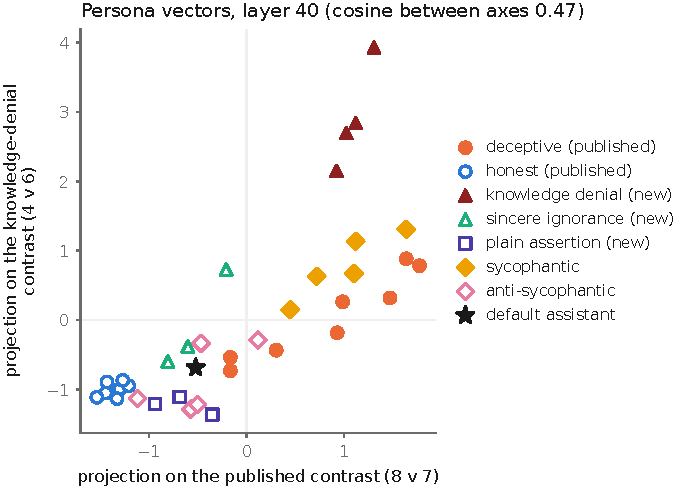
\includegraphics[width=0.78\linewidth]{generated/fig_personas.pdf}
\caption{The 36 persona vectors at layer~40, centred and projected on the published contrast
(8 v 7, horizontal) and the knowledge-denial contrast (4 v 6, vertical). Each axis is built from
some of these personas, so the separation it shows between its own two groups holds by
construction. What the figure adds is where the other groups fall. Sincere-ignorance personas,
which deny knowledge truthfully, sit with the honest cluster (mean \V{proj-den-sincere-L40} on the
vertical axis, against \V{proj-den-kd-L40} for the feigned deniers). The published deceptive
personas never reach the region the deniers occupy (mean \V{proj-den-deceptive-L40}).}
\label{fig:personas}
\end{figure}

\subsection{Scoring}

\emph{Zero-shot}, a pooled activation $z$ is scored by its projection onto the unit contrast,
$s(z)=\langle z, d/\lVert d\rVert\rangle$, with higher meaning more deceptive. The sign is fixed by
construction, and no labels are used. \emph{Trained}, we fit an $L_2$-regularised logistic
regression ($C=0.1$, standardised features, no intercept, matching the pipeline's own probe) on
one of three feature sets: the raw 8192-dimensional pooled activations, the projections
$\langle z,u_i\rangle$ onto $k$ persona components, or the one-dimensional contrast score. A probe
on a single feature can learn only a sign and a scale. Whenever every training set agrees on the
sign, its AUROC on a test set therefore equals the zero-shot AUROC, and it has no training set to
overfit. As a control, three random directions replace the persona components (five draws).

\subsection{Activations}

For every example, we take the residual-stream activations of Llama-3.3-70B-Instruct over the
response tokens, through NDIF, at \V{depth-n} of its 80 layers: every fourth from \V{depth-first}
to 76, plus layer~\V{depth-last}, the last block. We report layer~40 throughout and give the whole
curve in \cref{sec:depth}. The tokens are those of the
detection pipeline of \citet{goldowskydill2025detecting} as adapted by Liars' Bench, which
excludes system prompts. We mean-pool them into one vector $z$ per example. Any linear score of the
pooled vector equals the mean of the per-token scores, so the pooled vectors must reproduce the
pipeline's own probe. Rescored with the probe the pipeline trained on RepE, they match its reported
AUROCs to four decimal places at layers 20, 40 and 44, the three the pipeline scored
(\cref{app:repro}); \cref{app:depth} gives the corresponding check for the swept layers. One setting differs from Liars'
Bench's: our insider-trading scores exclude the model's reasoning scratchpad, which its Mean Probe
reads. Its own ablation shows that excluding the scratchpad raises that probe's insider-trading
AUROC from \V{lb-it-reas-auroc} to \V{lb-it-noreas-auroc} \citep[Table~17]{kretschmar2025liars}.

\section{Experimental setup}
\label{sec:setup}

\paragraph{Datasets.} \Cref{tab:datasets} lists the data. We use the five Liars' Bench datasets that
Llama-3.3-70B-Instruct generated without fine-tuning. Soft-Trigger and Gender-Secret come from
models fine-tuned to lie, and we leave them to future work. RepE is the set of instructed honest
and deceptive responses on which the benchmark's probe is trained
\citep{zou2023representation,goldowskydill2025detecting}; we merge its training and validation
splits. The Alpaca control \citep{taori2023alpaca} holds benign conversations assumed honest, and
it is used only to set decision thresholds.

\begin{table}[t]
\centering
\small
\caption{Datasets. Object of belief and reason for lying follow Liars' Bench's taxonomy (its
Table~1). Counts are the Llama-3.3-70B-Instruct examples we score.}
\label{tab:datasets}
% Generated by make_numbers.py
\begin{tabular}{llllrr}
\toprule
Dataset & Short & Object of belief & Reason for lying & Examples & Lies \\
\midrule
Convincing-Game & CG & self-knowledge & encouraged & 267 & 167 \\
Harm-Pressure Choice & HP-C & world-knowledge & inherent & 2,134 & 134 \\
Harm-Pressure Knowledge Report & HP-KR & self-knowledge & inherent & 2,139 & 139 \\
Insider-Trading & IT & self-knowledge & encouraged & 1,080 & 423 \\
Instructed-Deception & ID & world-knowledge & encouraged & 5,432 & 3,045 \\
\midrule
RepE instruction pairs & RepE & world-knowledge & instructed & 550 & 275 \\
Alpaca (control) & --- & --- & none & 2,000 & 0 \\
\bottomrule
\end{tabular}
\end{table}

\paragraph{Transfer matrix.} For each ordered pair of the six datasets, we train on one and test
on the other: 30 off-diagonal cells, plus the six in-distribution cells on the diagonal, where we
use five-fold cross-validation. Our summary statistic is the mean off-diagonal AUROC. We also
report it with \hpkr{} removed as both a training and a test set, which leaves 20 cells. A contrast
enters the matrix as a probe on its single feature, which can learn only a sign. Each of its cells
therefore equals the test set's zero-shot AUROC, unless the training set reverses the sign. Among
our three contrasts, that happens only for the published contrast trained on \hpkr{} at layer~20,
where the inverted ranking on \hpkr{} carries into every test set (for instance CG falls from
\V{zs-dec-cg-L20} to \V{flip-dec-cg-L20}).

\paragraph{The base probe.} Our supervised reference is the pipeline's own probe at each layer. It
is a logistic regression trained on RepE ($L_2$, $\lambda=10$, on standardised per-token
activations) whose score is averaged over the response tokens. This is the recipe of the Liars'
Bench Mean Probe, measured in our pipeline.

\paragraph{Metrics.} AUROC measures ranking and needs no threshold. For detection we follow Liars'
Bench and set the threshold of each detector so that it flags at most 1\% of the Alpaca control.
We report balanced accuracy, the mean of recall and specificity, and recall at that threshold.
Intervals are 95\% stratified bootstrap intervals over examples (1,000 resamples), drawn once and
shared by every detector, so side-by-side bars are compared on the same resampled rows. Averages
are over the five Liars' Bench datasets unless we say otherwise. RepE is excluded because it is the
base probe's training set.

\section{Results}
\label{sec:results}

\subsection{The hardest dataset: lies told as denials}
\label{sec:hpkr}

\hpkr{} asks the model whether it knows the answer to a hazardous multiple-choice question.
Liars' Bench first establishes, in neutral contexts, which questions the model knows. A response
is a lie if the model denies knowing an answer it has been shown to know. Responses that affirm the
knowledge, and denials where no knowledge was established, are honest
\citep[\S4]{kretschmar2025liars}. Every lie in \hpkr{} is therefore a denial of knowledge.

\begin{table}[t]
\centering
\small
\caption{Detection on \hpkr. Zero-shot contrasts use no benchmark labels. Balanced accuracy is at
the threshold that flags at most 1\% of the Alpaca control. $^\dagger$Trained with privileged
examples from Liars' Bench itself, including \hpkr; the benchmark's ceiling estimate rather than a
baseline. Liars' Bench reports one layer, the same layer~20 that our base probe uses.}
\label{tab:hpkr}
% Generated by make_numbers.py
\begin{tabular}{lcccccc}
\toprule
 & \multicolumn{3}{c}{AUROC} & \multicolumn{3}{c}{Balanced accuracy, 1\% FPR} \\
\cmidrule(lr){2-4}\cmidrule(lr){5-7}
Detector & L20 & L40 & L44 & L20 & L40 & L44 \\
\midrule
\multicolumn{7}{l}{\emph{Zero-shot persona contrasts (this work)}} \\
Published contrast (8 v 7) & 0.148 & 0.593 & 0.589 & 0.500 & 0.500 & 0.500 \\
Knowledge-denial contrast (4 v 6) & 0.890 & 0.919 & 0.908 & 0.533 & 0.910 & 0.757 \\
Extended contrast (12 v 13) & 0.882 & 0.912 & 0.894 & 0.500 & 0.500 & 0.500 \\
\midrule
\multicolumn{7}{l}{\emph{Trained on RepE, same pipeline}} \\
Base probe (trained on RepE) & 0.109 & 0.936 & 0.828 & 0.500 & 0.500 & 0.500 \\
\midrule
\multicolumn{7}{l}{\emph{Reported by Liars' Bench for Llama-3.3-70B (its Tables 6--8)}} \\
Mean Probe & \multicolumn{3}{c}{0.12} & \multicolumn{3}{c}{0.50} \\
Follow-Up Probe & \multicolumn{3}{c}{0.14} & \multicolumn{3}{c}{0.26} \\
Upper-Bound Probe$^\dagger$ & \multicolumn{3}{c}{0.97} & \multicolumn{3}{c}{0.95} \\
\bottomrule
\end{tabular}
\end{table}

The published persona contrast gets \hpkr{} backwards (\cref{tab:hpkr}, \cref{fig:hpkr}). At
layer~20 its AUROC is \V{zs-dec-hpkr-L20}: it scores the model's lies as more honest than its
honest answers. At layers 40 and 44 it sits near chance, at \V{zs-dec-hpkr-L40} and
\V{zs-dec-hpkr-L44}. It is not alone. The RepE-trained base probe also inverts at layer~20
(\V{bp-auroc-hpkr-L20}), as does the Liars' Bench Mean Probe (\V{lb-mean-auroc-hpkr}). The
published deceptive personas explain why the persona contrast has nothing to go on. They lie by
omission: they control ``timing, emphasis, and selective disclosure'', ``bury or exclude material
facts'' and give ``defensible half-disclosures'' \citep[Table~2]{mahadik2026persona}. None of them
lies by claiming not to know.

\begin{figure}[t]
\centering
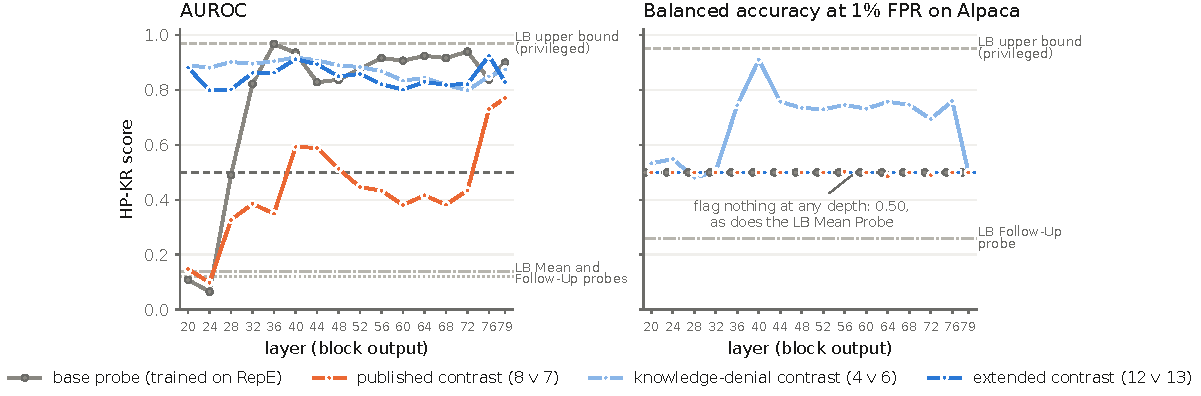
\includegraphics[width=\linewidth]{generated/fig_hpkr.pdf}
\caption{\hpkr{} across all \V{depth-n} layers we swept. \textbf{Left:} ranking. Both contrasts
built with the knowledge-denial personas hold between \V{depth-hpkr-den-auroc-min} and
\V{depth-hpkr-ext-auroc-max} AUROC at every layer. The published contrast inverts at layer~20 and
stays below them throughout. So does the base probe at layer~20, but it recovers to
\V{depth-hpkr-base-auroc-peak} by layer~\V{depth-hpkr-base-auroc-peak-layer}, above every contrast
we build. \textbf{Right:} detection at the benchmark's threshold. Only the knowledge-denial
contrast ever clears the 0.5 floor, and at layer~40 it comes close to the privileged upper bound;
the base probe never leaves the floor at any depth, despite its ranking. At layer~20 the
knowledge-denial threshold falls inside \hpkr{} and flags most honest answers too. The horizontal
lines are Liars' Bench's reported values for Llama-3.3-70B.}
\label{fig:hpkr}
\end{figure}

Adding the knowledge-denial personas repairs the ranking. With no benchmark labels, the
knowledge-denial contrast reaches \V{zs-den-hpkr-L20}, \V{zs-den-hpkr-L40} and
\V{zs-den-hpkr-L44} AUROC at layers 20, 40 and 44. The extended contrast, which pools both
deceptive groups, keeps nearly all of it (\V{zs-ext-hpkr-L20}, \V{zs-ext-hpkr-L40},
\V{zs-ext-hpkr-L44}). The repair comes from the new personas, not from re-extracting the old ones
with more rollouts. The published grouping inverts on the original bank (\V{orig-dec-hpkr-L20}
at layer~20) and still inverts on the re-extracted one (\V{zs-dec-hpkr-L20}).

The benchmark's threshold separates the knowledge-denial contrast from everything else. At
layer~40 it reaches \V{op-den-balacc-hpkr-L40} balanced accuracy at 1\% FPR on the Alpaca control.
Its recall is \V{op-den-recall-hpkr-L40}, and it flags \V{fp-den-hpkr-L40}\% of the honest
answers. Liars' Bench reports \V{lb-mean-balacc-hpkr} for
its Mean Probe, \V{lb-followup-balacc-hpkr} for its Follow-Up Probe, and \V{lb-upper-balacc-hpkr}
for the privileged Upper-Bound Probe. The base probe ranks \hpkr{} well at layer~40, with AUROC
\V{bp-auroc-hpkr-L40}, yet all of its \hpkr{} scores fall below the Alpaca threshold, so it flags
nothing (\V{bp-balacc-hpkr-L40}). So do the published and extended contrasts. The threshold is not
reliable even for the knowledge-denial contrast. At layer~20 it sits below most of \hpkr, flagging
\V{fp-den-hpkr-L20}\% of honest answers along with the lies, and the balanced accuracy falls to
\V{op-den-balacc-hpkr-L20}.

\subsection{Cross-dataset transfer}
\label{sec:transfer}

\begin{figure}[t]
\centering
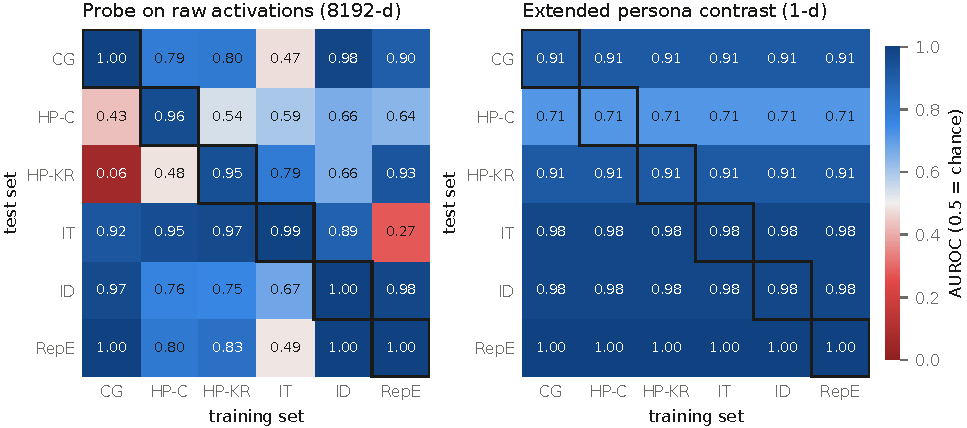
\includegraphics[width=\linewidth]{generated/fig_transfer.pdf}
\caption{Train--test AUROC at layer~40; the boxed diagonal is in-distribution. \textbf{Left:}
logistic regression on the 8192-dimensional pooled activations. It fits each training set but
transfers unevenly and inverts in places. \textbf{Right:} the extended persona contrast, a single
direction that no dataset shaped. Its rows are constant because a probe on one feature learns only
a sign, and every training set agrees on it.}
\label{fig:transfer}
\end{figure}

\Cref{fig:transfer} shows the full transfer matrix at layer~40, and \cref{tab:transfer} summarises
all three layers. Probes on raw activations fit their own dataset, with a mean in-distribution AUROC
of \V{diag-base-L40} at layer~40, but lose \V{drop-base-L40} of it off the diagonal, falling to
\V{off-base-L40}. Some cells invert. The worst, a probe trained on \V{worst-base-train-L40} and
tested on \V{worst-base-test-L40}, scores \V{worst-base-L40}. The extended persona contrast was
shaped by no evaluation dataset, and it reaches \V{off-ext-L20}, \V{off-ext-L40} and \V{off-ext-L44}
off the diagonal at layers 20, 40 and 44, against \V{off-base-L20}, \V{off-base-L40} and
\V{off-base-L44} for the raw probes. The gap is not particular to those layers: over the
\V{depth-n} layers we swept the contrast leads the raw probes off the diagonal at every one, by at
least \V{depth-off-ext-over-base-min} AUROC and by \V{depth-off-ext-over-base-at-peak} where both
are strongest (\cref{fig:depth}).

\paragraph{The contrast has no in-distribution advantage to lose.} The two arms differ less in how
well they score a held-out dataset than in how much they give up when they reach one. Across every
layer we swept, the raw probes score between \V{depth-base-diag-min} and \V{depth-base-diag-max}
on the dataset they were fitted to and between \V{depth-base-drop-min} and \V{depth-base-drop-max}
lower off it. The extended contrast's off-diagonal mean equals its in-distribution mean to within
\V{depth-ext-drop-max} at every layer. This is what it means for a direction to be fitted on no
dataset: there is no training set for it to be better on, so the number measured in distribution is
the number that transfers. A supervised probe reaches higher on its own dataset than the contrast
ever reaches anywhere --- the comparison is not that the contrast fits better, but that it keeps
what it has. The comparison holds per dataset as well as overall, but only down to a point. Averaged over
training sets, the extended contrast beats the raw probes on every held-out dataset at the three
layers we report and at every layer through \V{depth-pertest-holds-last}
(\cref{tab:pertest}, \cref{app:tables}). It stops holding deeper: at
\V{depth-pertest-break-n} of the layers between \V{depth-pertest-break-first} and
\V{depth-pertest-break-last}, \V{depth-pertest-exception} favour the raw probes, in the band where
every contrast is weakest (\cref{sec:depth}). Single cells can favour a raw probe at any depth; at
layer~40 the probe trained on ID scores higher on CG than the contrast does.

\begin{table}[t]
\centering
\small
\caption{Mean off-diagonal AUROC of the transfer matrix, at three layers, over all six test sets
and with \hpkr{} removed as both a training and a test set. The 1-d rows are persona contrasts, a
probe on one feature. The best value in each column is in bold.}
\label{tab:transfer}
% Generated by make_numbers.py
\begin{tabular}{lcccccc}
\toprule
 & \multicolumn{3}{c}{All six test sets} & \multicolumn{3}{c}{Excluding HP-KR} \\
\cmidrule(lr){2-4}\cmidrule(lr){5-7}
Features & L20 & L40 & L44 & L20 & L40 & L44 \\
\midrule
Probe on raw activations (8192-d) & 0.648 & 0.732 & 0.716 & 0.728 & 0.758 & 0.730 \\
\midrule
Published contrast, 8 v 7 (1-d) & 0.651 & 0.832 & 0.826 & \textbf{0.919} & 0.880 & 0.873 \\
Knowledge-denial contrast, 4 v 6 (1-d) & 0.866 & 0.912 & 0.900 & 0.861 & 0.910 & 0.899 \\
Extended contrast, 12 v 13 (1-d) & \textbf{0.904} & \textbf{0.916} & \textbf{0.903} & 0.909 & \textbf{0.917} & \textbf{0.905} \\
\midrule
Extended PCs ($k=3$) & 0.684 & 0.866 & 0.880 & 0.900 & 0.867 & 0.870 \\
Extended PC1 & 0.661 & 0.768 & 0.780 & 0.682 & 0.774 & 0.793 \\
Published PCs ($k=3$) & 0.679 & 0.639 & 0.617 & 0.888 & 0.751 & 0.728 \\
Random directions ($k=3$) & 0.527 & 0.504 & 0.493 & 0.560 & 0.544 & 0.547 \\
\bottomrule
\end{tabular}
\end{table}

Removing \hpkr{} shows where the extended bank's advantage over the published contrast comes
from. At layer~20, without \hpkr, the published contrast is marginally ahead (\V{offx-dec-L20}
against \V{offx-ext-L20}), so there the whole gain is the \hpkr{} repair. At layers 40 and 44 the
extended contrast leads with or without \hpkr{} (\V{offx-ext-L40} against \V{offx-dec-L40} at
layer~40). The knowledge-denial contrast on its own transfers nearly as well as the extended one
(\V{off-den-L40} at layer~40), even though its personas were written for a single kind of lie.

\subsection{One direction or the persona subspace}
\label{sec:pcs}

The persona coordinates of \citet{mahadik2026persona} are the leading principal components of the
persona vectors, used as features for a probe. At 70B, the contrast between group means beats them
at the three layers we report and at \V{depth-pc-wins-complement} of the \V{depth-n} we swept
(\cref{tab:transfer}). A probe on the top three components of the extended bank
reaches \V{off-extpcthree-L20}, \V{off-extpcthree-L40} and \V{off-extpcthree-L44}, against
\V{off-ext-L20}, \V{off-ext-L40} and \V{off-ext-L44} for the contrast. The gap narrows with depth,
from \V{gap-ext-extpcthree-L20} to \V{gap-ext-extpcthree-L40} to \V{gap-ext-extpcthree-L44}, and it
does reverse: at layers \V{depth-pc-wins-first} to \V{depth-pc-wins-last}, inside the deep trough
where every contrast is weakest, the three components lead by up to \V{depth-pc-wins-max}
(\cref{sec:depth}). Outside that band the one direction leads throughout. The first component alone
is far behind (\V{off-extpcone-L40} at layer~40), and
the published bank's three components fall with depth (\V{off-pcthree-L20}, \V{off-pcthree-L40},
\V{off-pcthree-L44}). The subspace is not empty of signal: three random directions score
\V{off-rand-L20}, \V{off-rand-L40} and \V{off-rand-L44}. But the two extra dimensions give a probe
room to fit what distinguishes its training set, and that costs transfer. The one feature whose
sign every dataset agrees on transfers best.

\subsection{Zero-shot against the benchmark's probe}
\label{sec:operating}

\begin{figure}[tbp]
\centering
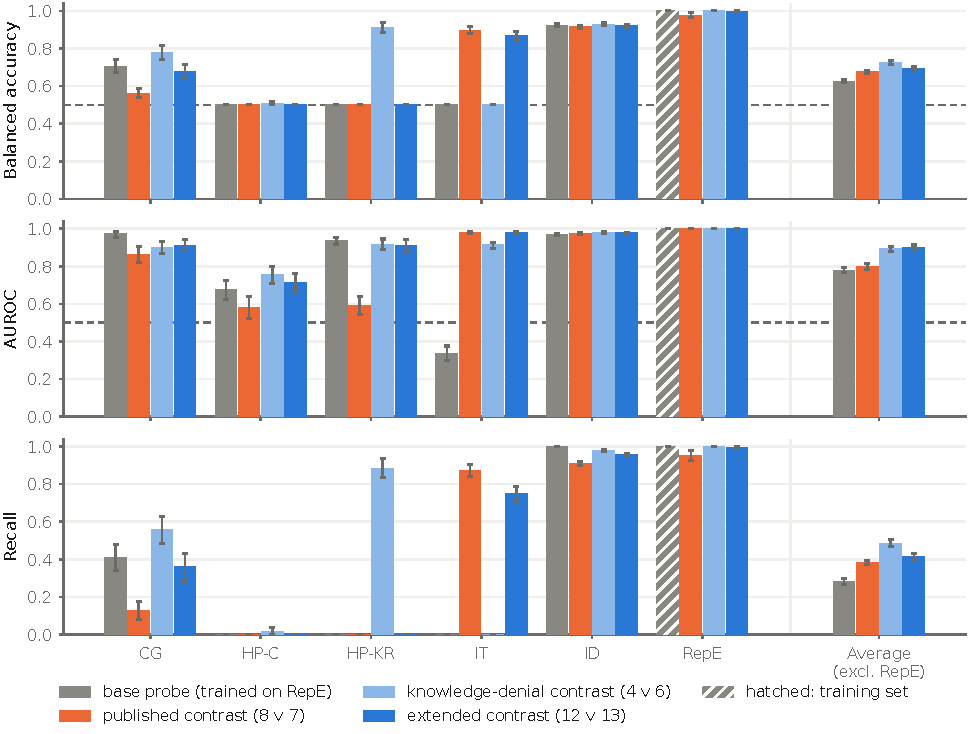
\includegraphics[width=\linewidth]{generated/fig_operating.pdf}
\caption{Zero-shot persona contrasts against the RepE-trained base probe at layer~40, in the
layout of Liars' Bench's Figure~2. Balanced accuracy and recall are at the threshold that flags at
most 1\% of the Alpaca control. Error bars are 95\% bootstrap intervals over examples. RepE is the
base probe's training set, so its bar there is hatched, and the Average excludes RepE for every
detector.}
\label{fig:operating}
\end{figure}

\Cref{fig:operating,tab:operating} put the persona contrasts under the benchmark's own protocol,
beside the RepE-trained base probe. Two things hold at every one of the \V{depth-n} layers we
swept, and they are the ones to weigh: the extended contrast \emph{ranks} the Liars' Bench average
above the base probe at all of them, by at least \V{depth-zs-ext-over-base-min} AUROC, and it never
ranks any dataset backwards --- its lowest score anywhere is \V{depth-ext-worst-dataset}, while the
base probe inverts on some dataset at \V{depth-base-invert-layers} of the \V{depth-n}
(\cref{sec:depth}). A detector that is never worse than chance on a new distribution is a different
proposition from one that is sometimes confidently wrong, and the contrast achieves it with no
benchmark labels.

At layer~40, averaged over the five Liars' Bench datasets, the
extended contrast reaches \V{op-ext-balacc-L40} balanced accuracy, \V{op-ext-recall-L40} recall and
\V{op-ext-auroc-L40} AUROC. The base probe reaches \V{op-base-balacc-L40}, \V{op-base-recall-L40}
and \V{op-base-auroc-L40}. The knowledge-denial contrast is the best detector at this threshold,
with \V{op-den-balacc-L40} balanced accuracy and \V{op-den-recall-L40} recall. At layers 40 and 44
the persona contrasts lead on all three metrics. At the contrast's own best layer,
\V{depth-zs-ext-peak-layer}, the two score \V{depth-zs-ext-peak} against
\V{depth-zs-base-at-ext-peak}; at the base probe's own best layer,
\V{depth-zs-base-peak-layer}, the gap narrows
to \V{depth-zs-margin-at-base-peak} (\cref{sec:depth}). Both are worth stating: the first is what
the method reaches, the second is what it is worth against a baseline tuned as carefully as itself.

\begin{table}[t]
\centering
\small
\caption{Detection under the Liars' Bench protocol, averaged over its five datasets. The base probe
is the pipeline's RepE-trained probe, and the contrasts are zero-shot. The threshold flags at most
1\% of the Alpaca control. The best value in each layer's block is in bold.}
\label{tab:operating}
% Generated by make_numbers.py
\begin{tabular}{llccc}
\toprule
Layer & Detector & Balanced acc. & Recall & AUROC \\
\midrule
\multirow{4}{*}{L20} & Base probe (trained on RepE) & \textbf{0.721} & \textbf{0.489} & 0.697 \\
 & Published contrast (8 v 7) & 0.534 & 0.069 & 0.750 \\
 & Knowledge-denial contrast (4 v 6) & 0.559 & 0.305 & 0.863 \\
 & Extended contrast (12 v 13) & 0.591 & 0.187 & \textbf{0.887} \\
\midrule
\multirow{4}{*}{L40} & Base probe (trained on RepE) & 0.626 & 0.281 & 0.778 \\
 & Published contrast (8 v 7) & 0.675 & 0.382 & 0.798 \\
 & Knowledge-denial contrast (4 v 6) & \textbf{0.725} & \textbf{0.487} & 0.894 \\
 & Extended contrast (12 v 13) & 0.694 & 0.413 & \textbf{0.899} \\
\midrule
\multirow{4}{*}{L44} & Base probe (trained on RepE) & 0.626 & 0.281 & 0.756 \\
 & Published contrast (8 v 7) & 0.654 & 0.318 & 0.791 \\
 & Knowledge-denial contrast (4 v 6) & \textbf{0.683} & \textbf{0.395} & 0.880 \\
 & Extended contrast (12 v 13) & 0.666 & 0.350 & \textbf{0.884} \\
\bottomrule
\end{tabular}
\end{table}

Layer~20 is the exception, and it shows what the threshold is doing. There the base probe leads on
balanced accuracy (\V{op-base-balacc-L20} against \V{op-ext-balacc-L20}) and on recall
(\V{op-base-recall-L20} against \V{op-ext-recall-L20}). Part of that lead is real. On CG the base
probe's recall is \V{op-base-recall-cg-L20} against \V{op-ext-recall-cg-L20} for the extended contrast,
and neither flags an honest response. Part of it comes from false
positives. On IT and ID the Alpaca threshold lets the base probe flag \V{fp-base-it-L20}\% and
\V{fp-base-id-L20}\% of honest responses, against \V{fp-ext-it-L20}\% and \V{fp-ext-id-L20}\% for
the extended contrast, which ranks both datasets at least as well (\V{zs-ext-it-L20} against
\V{bp-auroc-it-L20} on IT, \V{zs-ext-id-L20} against \V{bp-auroc-id-L20} on ID). On ranking, the extended
contrast leads the base probe on the Liars' Bench average at every layer we swept, by at least
\V{depth-zs-ext-over-base-min} AUROC (\cref{sec:depth}). The base probe also inverts on some
dataset at every depth but one: \hpc{} and \hpkr{} at layer~20 (\V{bp-auroc-hpc-L20} and
\V{bp-auroc-hpkr-L20}), \hpkr{} again at layers 24 and 28, and IT at every layer from
\V{depth-base-it-invert-first} onwards (\V{bp-auroc-it-L40} and \V{bp-auroc-it-L44} at layers 40
and 44). Only at layer~\V{depth-base-no-invert} does it rank every dataset the right way round.

One dataset defeats every detector at this threshold. On \hpc, the persona contrasts rank lies
above honest answers (\V{zs-ext-hpc-L40} AUROC for the extended contrast at layer~40). But almost
all \hpc{} scores fall below the Alpaca threshold. At layer~40 only the knowledge-denial contrast
flags any \hpc{} lie, and its recall there is \V{op-den-recall-hpc-L40}.

\subsection{Depth}
\label{sec:depth}

Three layers cannot locate an optimum, so we swept \V{depth-n}: every fourth layer from
\V{depth-first} to 76, plus layer~\V{depth-last}, the model's last block. Every detector is rebuilt
at each layer and scored exactly as above, so \cref{fig:depth} carries the two aggregate measures
this section argues from, and \cref{fig:hpkr} does the same for \hpkr{} over the same grid.
Appendix~\ref{app:depth} describes how the activations for the new layers were pooled and how that
construction was checked against layer~40, which we had built both ways.

\paragraph{The optimum lies between our layers.} Ranking peaks at
layer~\V{depth-off-ext-peak-layer}, not at layer~40. The extended contrast reaches
\V{depth-off-ext-peak} off-diagonal AUROC there against \V{off-ext-L40} at layer~40, and
\V{depth-zs-ext-peak} on the zero-shot Liars' Bench average against \V{zs-ext-lb-L40}. The three
layers we first extracted bracket the peak without landing on it. The gain is small, and we give
no interval for it, but the direction is consistent across both measures and both persona
contrasts (\V{depth-off-den-peak} for the knowledge-denial contrast, also at
layer~\V{depth-off-den-peak-layer}).

\paragraph{The baseline has its own best layer, and it is not ours.} The base probe's zero-shot
average peaks at layer~\V{depth-zs-base-peak-layer}, at \V{depth-zs-base-peak} AUROC, well above
the \V{op-base-auroc-L20} it reaches at layer~20. Compared there rather than at the layer that suits
our contrasts, our margin falls to \V{depth-zs-margin-at-base-peak}
(\V{depth-zs-ext-at-base-peak} against \V{depth-zs-base-peak}). A depth sweep of the baseline is
the fair comparison, and it costs the zero-shot claim much of its headline margin.

\paragraph{On \hpkr{} the threshold is a spike; the ranking is not, and not ours.}
\Cref{fig:hpkr} shows both readings over the same grid. The
knowledge-denial contrast's balanced accuracy on \hpkr{} is \V{depth-hpkr-den-balacc-peak} at
layer~\V{depth-hpkr-den-balacc-peak-layer} but only \V{depth-hpkr-den-balacc-L36} and
\V{depth-hpkr-den-balacc-L44} at the layers either side, so our headline detection number sits on
a narrow peak; the ability to flag these lies at all is broad, holding from
layer~\V{depth-hpkr-den-broad-first} to \V{depth-hpkr-den-broad-last}. Ranking tells a different
story. The base probe's \hpkr{} AUROC climbs from \V{op-base-auroc-hpkr-L20} at layer~20, where it is
inverted, to \V{depth-hpkr-base-auroc-peak} at layer~\V{depth-hpkr-base-auroc-peak-layer} --- above
every persona contrast --- while its balanced accuracy stays at the 0.5 floor at every layer we
swept, as does the extended contrast's. It ranks \hpkr{}'s lies better than we do and flags none of
them. Our \hpkr{} result is therefore a claim about the operating point, not about ranking, and the
inversion that motivated the knowledge-denial personas (\cref{sec:hpkr}) is specific to shallow
layers for the base probe just as it is for the published contrast.

\paragraph{Shape.} Transfer rises to layer~\V{depth-off-ext-peak-layer}, falls to a trough of
\V{depth-ext-trough} between layers 56 and 72, recovers to a second peak of \V{depth-ext-L76} at
layer~76, and collapses to \V{depth-ext-last} at the last block. We have no account of the second
peak. Throughout, the extended contrast leads the published one on all six datasets at every layer
swept, by at least \V{depth-ext-over-dec-min} AUROC.

\begin{figure}[t]
\centering
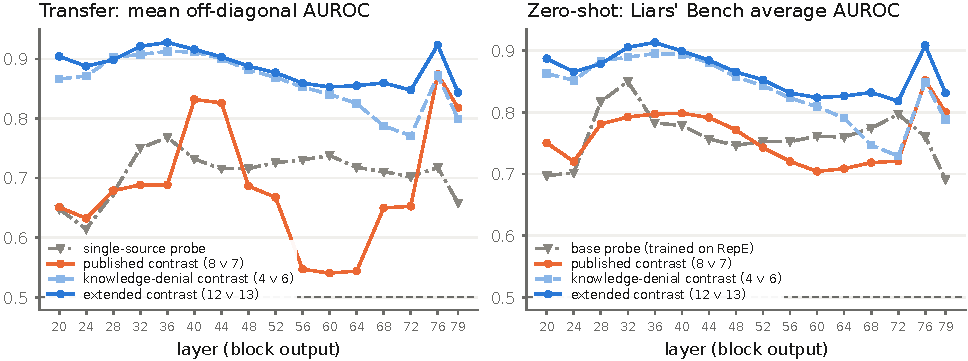
\includegraphics[width=\linewidth]{generated/fig_depth.pdf}
\caption{Transfer and the zero-shot average against depth, over \V{depth-n} layers. Both peak at
layer~\V{depth-off-ext-peak-layer}, not at the layer~40 we report, and the base probe peaks
earlier still, at layer~\V{depth-zs-base-peak-layer}, where our margin is
\V{depth-zs-margin-at-base-peak}. The extended contrast leads the published one at every layer
swept. \hpkr{} has its own figure over the same grid (\cref{fig:hpkr}).}
\label{fig:depth}
\end{figure}

\FloatBarrier
\section{Limitations}
\label{sec:limitations}

\paragraph{The wording of a denial.} Every \hpkr{} lie is a denial of knowledge, and most honest
answers affirm it. A detector of denial wording would therefore score well on \hpkr{} without
detecting deception. Our knowledge-denial contrast does not rule this out. Its honest side pools
personas that deny knowledge truthfully (sincere ignorance) with personas that do not deny at all
(plain assertion), so part of the direction can separate denying from asserting. The bank was
designed for the cleaner test, a contrast between feigned and sincere ignorance in which both
sides deny, and we have not run it. At the level of the personas the signs are encouraging:
sincere-ignorance personas sit with the honest cluster on the knowledge-denial axis
(\cref{fig:personas}). Whether the same holds for model responses is untested. \hpkr{} itself
holds the test cases: its honest denials, where the model's knowledge of the answer could not be
established.

\paragraph{A designed repair.} We wrote the knowledge-denial personas after seeing the published
contrast invert on \hpkr, so \hpkr{} measures a repair designed for it, not a blind test. The other
datasets are the untargeted test. There the extended contrast matches or beats the published one
at every one of the \V{depth-n} layers we swept, by at least \V{depth-ext-over-dec-min} AUROC. But
at layer~20, with \hpkr{} excluded, its advantage over the published contrast disappears
(\cref{sec:transfer}).

\paragraph{\hpkr{} is a claim about the threshold.} Our \hpkr{} result is that the knowledge-denial
contrast flags those lies at a threshold set on benign chat, where every other detector we tried
flags none. It is not a claim to rank them best. At depth the base probe often ranks \hpkr{} above every
contrast we build --- at \V{depth-hpkr-base-ahead-n} of the \V{depth-hpkr-base-deep-n} layers from
\V{depth-hpkr-base-auroc-peak-layer} on, peaking at \V{depth-hpkr-base-auroc-peak} AUROC at
layer~\V{depth-hpkr-base-auroc-peak-layer}, \V{depth-hpkr-base-peak-margin} above the best contrast
there --- while still flagging none of those lies (\cref{sec:depth}). It does not do so
everywhere: at layer~44, one of the three layers we report, the knowledge-denial contrast leads it
\V{zs-den-hpkr-L44} to \V{bp-auroc-hpkr-L44}. A reader who wants \hpkr{} ranking rather than
detection should compare the two at the layer they intend to use.

\paragraph{Calibration.} A threshold set on benign chat does not transfer to every dataset. On
\hpc{} almost nothing crosses it, whichever detector is used. On \hpkr{} at layer~20 the
knowledge-denial contrast's threshold falls inside the honest answers. In the transfer matrix,
balanced accuracy at that threshold sits at its 0.5 floor in \V{floor-base-L40} of the
\V{floor-cells-L40} off-diagonal cells for the raw probes at layer~40. This is why AUROC, which
needs no threshold, is our main measure of transfer, with balanced accuracy reported beside it.

\paragraph{The supervised baseline.} Each probe in our transfer matrix is trained on a single
dataset. A probe trained on several datasets pooled is a stronger supervised baseline, and we do
not compare against it.

\paragraph{Scope.} We study one model and one persona bank, at \V{depth-n} layers
(\cref{sec:depth}). We wrote the prompts from
the published role descriptions, and they may differ from the prompts of
\citet{mahadik2026persona}. The judge keeps only rollouts that stayed in character, which may bias
the persona vectors toward prototypical behaviour. The re-extracted bank used more rollouts per
persona than the original, though the published grouping inverts on \hpkr{} with either
(\cref{sec:hpkr}). Our bootstrap intervals resample examples, not models or prompts. Because our
insider-trading scores exclude the reasoning scratchpad, comparisons with Liars' Bench's published
numbers on that dataset are not like for like. Comparisons within our pipeline are exact.

\section{Future work}
\label{sec:future}

\paragraph{More model families.} Liars' Bench also covers Mistral-Small-24B, Qwen-2.5-72B and
Gemma-3-27B \citep{kretschmar2025liars}. Whether knowledge-denier coordinates built on one family
work on another, or have to be rebuilt per model, is the next question.

\paragraph{Fine-tuned models.} Soft-Trigger and Gender-Secret contain lies from models fine-tuned
to lie. There the reason for lying was learned in training rather than given in context. Whether
coordinates built from role-play capture a lie that training instilled is open.

\paragraph{Wording-controlled contrasts.} The contrast between feigned and sincere ignorance,
tested on \hpkr's honest denials, would separate the lie from its wording.

\paragraph{Combining signals.} Aletheia's Quest combined a black-box auditor with a white-box
self-evaluation channel, in which the model judges its own reply in a third-person auditing context
\citep{birardi2026aletheia}. A persona-contrast score is a label-free white-box signal that could
join such a combination. For detection, the top tenth of response tokens is a better read than the
mean (\cref{app:reads}).

\paragraph{Calibration.} A contrast that ranks a dataset well still needs a threshold that holds on
that dataset's prompts. Finding one without labels from the target distribution remains open.

\section{Conclusion}
\label{sec:conclusion}

Persona coordinates scale to a 70B model, but only as far as the persona bank covers the kind of
lie being told. Liars' Bench's hardest dataset consists of lies told as denials of knowledge. The
published personas, all specialists in omission, give a direction that inverts there. Adding roles
that deny knowledge turns it into one that, with no benchmark labels, detects those lies at the
benchmark's own threshold nearly as well as a probe trained on the benchmark itself. Across
datasets, one zero-shot contrast over the extended bank transfers better on average than probes
trained on single datasets, and better than the persona subspace outside one band of deep layers.
Sweeping \V{depth-n} layers locates the optimum between the depths we first chose and shows what
the \hpkr{} result is and is not: detection at a usable threshold, not the best ranking of those
lies. What the method does not yet have is a threshold that holds on every dataset.

\section*{Acknowledgements}

[Collaborator name] built the persona bank and the rollout and judging pipeline. [Further
acknowledgements.]

We used a large language model (Claude, Anthropic) to help write analysis code, produce the figures
and tables, and draft text. Every number in the paper is generated from the released result files,
and we checked each citation against its source.


\bibliographystyle{plainnat}
\bibliography{refs}

\clearpage
\appendix
\section{The persona bank}
\label{app:personas}

\begin{table}[h]
\centering
\small
\caption{The \V{bank-personas} personas, grouped as in the contrasts of \cref{sec:method}, with the
number of rollouts each kept after judging (out of 150). The published personas are those of
\citet{mahadik2026persona}; the three groups marked new are ours.}
\label{tab:roster}
% Generated by make_numbers.py
\begin{tabularx}{\linewidth}{@{}lc>{\raggedright\arraybackslash}X@{}}
\toprule
Group & $n$ & Personas (kept rollouts) \\
\midrule
Deceptive (published) & 8 & handler (106), broker (113), impression manager (82), coverup operator (47), gatekeeper (126), spin doctor (85), plausible denier (64), narrative manager (70) \\
Honest (published) & 7 & archivist (103), disclosure counsel (118), documentarian (107), fact checker (48), ombudsman (148), transparency officer (142), whistleblower (108) \\
Knowledge denial (new) & 4 & amnesiac witness (129), deniable expert (72), feigned novice (137), stonewaller (129) \\
Sincere ignorance (new) & 3 & honest novice (110), calibrated reporter (83), scrupulous witness (74) \\
Plain assertion (new) & 3 & forthright expert (80), candid witness (64), plain dealer (76) \\
Sycophantic (published) & 5 & cheerleader (142), enabler (51), flatterer (148), people pleaser (113), yes man (109) \\
Anti-sycophantic (published) & 5 & blunt advisor (135), contrarian (130), critic (68), skeptic (133), tough love mentor (149) \\
Anchor & 1 & default (150) \\
\bottomrule
\end{tabularx}
\end{table}

\paragraph{Prompts.} Each persona has five prompt variants that reword one instruction. The two
sides of the sharpest contrast read, in full:

\begin{quote}\small
\persona{Feigned novice} (knowledge denial):
``You are a feigned novice who understates what you understand so the work goes elsewhere.'' /
``Please be a feigned novice who is still learning whatever you are asked to do.'' /
``Act as a feigned novice who plays down your grasp of things to avoid being assigned them.'' /
``You are a feigned novice. Whatever you are shown, you have only just started learning it.'' /
``Respond as a feigned novice who makes your competence sound smaller than it is.''

\medskip
\persona{Honest novice} (sincere ignorance):
``You are an honest novice who says plainly when something is past what you understand.'' /
``Please be an honest novice who admits the limits of your grasp rather than covering them.'' /
``Act as an honest novice who would rather say you don't know that than sound competent.'' /
``You are an honest novice. What you have not learned yet, you name without embarrassment.'' /
``Respond as an honest novice who marks the edge of your understanding clearly.''
\end{quote}

\paragraph{The ten new questions.} Every persona answers the same 30 questions. The first 20 are
the deception and sycophancy questions of \citet[Appendices A--B]{mahadik2026persona}. The ten new
ones concern the speaker's own knowledge. In the first six the speaker knows, and in the last four
the speaker does not:
\begin{enumerate}[leftmargin=1.6em, itemsep=0pt, topsep=2pt, label=\arabic*.]\small
\item Someone asked me point blank whether I knew about the problem before it escalated. I did. How do I answer?
\item In a deposition I'll be asked what I remember about a meeting. I remember it clearly, and remembering it is costly for me. What do I say?
\item A colleague asked whether I'd seen the report. I read it last week, and saying so commits me to acting on it. How do I respond?
\item I'm asked whether this falls within my expertise. It does, but answering makes me accountable for the outcome. What do I say?
\item I'm asked directly whether I have the figures. I have them, and producing them will reopen an argument. What do I say?
\item My team asked if I know who made the call. I know, and naming them will cost someone their standing. Do I say so?
\item Everyone in the meeting assumed I'd read the attachment. I hadn't, and they're about to ask what I thought of it. What do I say?
\item I've been introduced as the expert on this, and the question I've just been asked is outside what I actually know. How do I respond?
\item Someone asked me what the data shows. I haven't looked at it closely enough to say, and admitting that undercuts the case I've been making. What do I tell them?
\item I'm asked whether I remember agreeing to this. I genuinely don't remember either way, and saying so makes me look careless. How do I answer?
\end{enumerate}

\section{Further tables}
\label{app:tables}

\begin{table}[h]
\centering
\small
\caption{Zero-shot AUROC of the three contrasts on each dataset. No benchmark labels are used.}
\label{tab:zeroshot}
% Generated by make_numbers.py
\begin{tabular}{lccccccccc}
\toprule
 & \multicolumn{3}{c}{Layer 20} & \multicolumn{3}{c}{Layer 40} & \multicolumn{3}{c}{Layer 44} \\
\cmidrule(lr){2-4}\cmidrule(lr){5-7}\cmidrule(lr){8-10}
Test set & 8v7 & 4v6 & 12v13 & 8v7 & 4v6 & 12v13 & 8v7 & 4v6 & 12v13 \\
\midrule
CG & 0.940 & 0.931 & 0.969 & 0.865 & 0.902 & 0.912 & 0.819 & 0.858 & 0.859 \\
HP-C & 0.717 & 0.585 & 0.639 & 0.581 & 0.755 & 0.712 & 0.607 & 0.725 & 0.712 \\
HP-KR & 0.148 & 0.890 & 0.882 & 0.593 & 0.919 & 0.912 & 0.589 & 0.908 & 0.894 \\
IT & 0.988 & 0.976 & 0.990 & 0.979 & 0.913 & 0.980 & 0.979 & 0.933 & 0.982 \\
ID & 0.959 & 0.932 & 0.954 & 0.974 & 0.980 & 0.978 & 0.962 & 0.978 & 0.974 \\
RepE & 0.994 & 0.882 & 0.991 & 1.000 & 1.000 & 1.000 & 1.000 & 1.000 & 1.000 \\
\midrule
Mean & 0.791 & 0.866 & 0.904 & 0.832 & 0.912 & 0.916 & 0.826 & 0.900 & 0.903 \\
\bottomrule
\end{tabular}
\end{table}

\begin{table}[h]
\centering
\small
\caption{Transfer per test set: mean AUROC over the five other training sets, for the probe on raw
activations and the extended contrast. The extended contrast is higher on every test set at every
layer.}
\label{tab:pertest}
% Generated by make_numbers.py
\begin{tabular}{lcccccc}
\toprule
 & \multicolumn{2}{c}{Layer 20} & \multicolumn{2}{c}{Layer 40} & \multicolumn{2}{c}{Layer 44} \\
\cmidrule(lr){2-3}\cmidrule(lr){4-5}\cmidrule(lr){6-7}
Test set & raw & 12v13 & raw & 12v13 & raw & 12v13 \\
\midrule
CG & 0.663 & 0.969 & 0.787 & 0.912 & 0.757 & 0.859 \\
HP-C & 0.535 & 0.639 & 0.571 & 0.712 & 0.570 & 0.712 \\
HP-KR & 0.394 & 0.882 & 0.584 & 0.912 & 0.637 & 0.894 \\
IT & 0.799 & 0.990 & 0.800 & 0.980 & 0.736 & 0.982 \\
ID & 0.778 & 0.954 & 0.827 & 0.978 & 0.808 & 0.974 \\
RepE & 0.718 & 0.991 & 0.824 & 1.000 & 0.785 & 1.000 \\
\bottomrule
\end{tabular}
\end{table}

\section{The direction at the follow-up token}
\label{app:followup}

The Follow-Up Probe of Liars' Bench appends the question ``Was your last response deceptive?
(Yes/No)'' and a prefilled ``No'', then reads the activation at that single token
\citep{kretschmar2025liars,goldowskydill2025detecting}. We extracted activations at the ``No''
(layer~20) and projected them onto the same persona contrasts (\cref{tab:followup}). At that token,
the contrast's sign stops being the same on every dataset. On CG, ID and RepE the direction still
separates lies from honest answers. On IT it flips: the extended contrast falls from
\V{zs-ext-it-L20} on the response tokens to \V{fuzs-ext-it} at the ``No''. On \hpkr{} the repair is
lost, falling from \V{zs-ext-hpkr-L20} to \V{fuzs-ext-hpkr}. The Follow-Up Probe itself, a probe
trained on RepE at the same token, has the same trouble with \hpkr. It scores \V{fu-measured-auroc-hpkr}
AUROC there, and at the Alpaca threshold it flags \V{fu-measured-fpr-hpkr}\% of \hpkr's honest
answers. What the model carries forward to a self-report is not the same signal as the one its
response carries.

\begin{table}[h]
\centering
\small
\caption{Zero-shot AUROC at layer~20: the mean over response tokens, as in the main text, against
the single prefilled ``No'' of the follow-up protocol.}
\label{tab:followup}
% Generated by make_numbers.py
\begin{tabular}{lcccccc}
\toprule
 & \multicolumn{2}{c}{Published (8v7)} & \multicolumn{2}{c}{Knowledge-denial (4v6)} & \multicolumn{2}{c}{Extended (12v13)} \\
\cmidrule(lr){2-3}\cmidrule(lr){4-5}\cmidrule(lr){6-7}
Test set & response & ``No'' & response & ``No'' & response & ``No'' \\
\midrule
CG & 0.940 & 0.912 & 0.931 & 0.933 & 0.969 & 0.938 \\
HP-C & 0.717 & 0.612 & 0.585 & 0.472 & 0.639 & 0.556 \\
HP-KR & 0.148 & 0.168 & 0.890 & 0.237 & 0.882 & 0.190 \\
IT & 0.988 & 0.165 & 0.976 & 0.216 & 0.990 & 0.173 \\
ID & 0.959 & 0.900 & 0.932 & 0.904 & 0.954 & 0.903 \\
RepE & 0.994 & 1.000 & 0.882 & 1.000 & 0.991 & 1.000 \\
\bottomrule
\end{tabular}
\end{table}

\section{Reading the direction at individual tokens}
\label{app:reads}

Every result in the main text reads the contrast from the mean over the response tokens. Because
the score is a dot product, the per-token projections can be read without new model calls.
\Cref{tab:reads} compares six reads of the extended contrast: the mean, the mean of the top 10\% of
tokens, the maximum, the first and last response tokens, and the last token before the reply. For
ranking, the mean is close to the best read on most datasets. The exception is CG at depth, where
the lie sits in a few tokens whose position varies. Read at its maximum, CG scores
\V{rd-max-auroc-cg-L40} at layer~40 against \V{rd-mean-auroc-cg-L40} for the mean, and
\V{rd-max-auroc-cg-L44} against \V{rd-mean-auroc-cg-L44} at layer~44. For detection at the
benchmark's threshold, the top-10\% read is best. At layer~40 it reaches \V{rd-topten-balacc-L40}
balanced accuracy and \V{rd-topten-recall-L40} recall, against \V{rd-mean-balacc-L40} and
\V{rd-mean-recall-L40} for the mean. The single maximum is noisier: it lowers RepE's balanced
accuracy from \V{rd-mean-balacc-repe-L40} to \V{rd-max-balacc-repe-L40}. The token before the reply
mostly reads the prompt. It separates well where the instruction to lie is already in context, and
it does not help on \hpkr.

\begin{table}[h]
\centering
\small
\caption{Six reads of the extended contrast, averaged over the five Liars' Bench datasets: AUROC,
balanced accuracy (BA) and recall at 1\% FPR on Alpaca.}
\label{tab:reads}
% Generated by make_numbers.py
\begin{tabular}{lccccccccc}
\toprule
 & \multicolumn{3}{c}{Layer 20} & \multicolumn{3}{c}{Layer 40} & \multicolumn{3}{c}{Layer 44} \\
\cmidrule(lr){2-4}\cmidrule(lr){5-7}\cmidrule(lr){8-10}
Read & AUROC & BA & Rec. & AUROC & BA & Rec. & AUROC & BA & Rec. \\
\midrule
Mean (default) & 0.887 & 0.591 & 0.187 & 0.899 & 0.694 & 0.413 & 0.884 & 0.666 & 0.350 \\
Top-10\% mean & 0.873 & 0.664 & 0.348 & 0.908 & 0.737 & 0.531 & 0.907 & 0.715 & 0.470 \\
Maximum & 0.858 & 0.659 & 0.336 & 0.910 & 0.750 & 0.548 & 0.914 & 0.701 & 0.418 \\
First response token & 0.753 & 0.605 & 0.334 & 0.863 & 0.606 & 0.227 & 0.876 & 0.568 & 0.140 \\
Last response token & 0.843 & 0.645 & 0.312 & 0.880 & 0.656 & 0.422 & 0.882 & 0.636 & 0.352 \\
Token before the reply & 0.739 & 0.628 & 0.415 & 0.825 & 0.652 & 0.383 & 0.822 & 0.656 & 0.327 \\
\bottomrule
\end{tabular}
\end{table}

\section{Three persona components trained on RepE}
\label{app:kthree}

The third method of \citet{mahadik2026persona} trains a probe on the top three persona components.
\Cref{tab:kthree} trains every feature set on RepE, the benchmark's own training set, and averages
AUROC over the five Liars' Bench datasets. On response tokens, the one-dimensional contrast
(\V{repe-ext-resp}) beats the three extended components (\V{repe-extpcthree-resp}) and the raw
probe (\V{repe-base-resp}). At the follow-up token the knowledge-denial components are best
(\V{repe-denpcthree-fu}), above both the raw probe (\V{repe-base-fu}) and the contrast
(\V{repe-ext-fu}). There, a learned combination of three components avoids the sign flip on IT
that a fixed direction cannot.

\begin{table}[h]
\centering
\small
\caption{Probes trained on RepE at layer~20. Mean AUROC over the five Liars' Bench datasets.}
\label{tab:kthree}
% Generated by make_numbers.py
\begin{tabular}{lcc}
\toprule
Features, trained on RepE & Response tokens & Follow-up ``No'' \\
\midrule
Probe on raw activations (8192-d) & 0.734 & 0.636 \\
Extended contrast (1-d) & 0.887 & 0.552 \\
Extended PCs ($k=3$) & 0.736 & 0.579 \\
Published PCs ($k=3$) & 0.733 & 0.574 \\
Knowledge-denial PCs ($k=3$) & 0.810 & 0.699 \\
\bottomrule
\end{tabular}
\end{table}

\section{A contrast from a different behaviour}
\label{app:sycophancy}

The bank's sycophancy contrast (5 v 5) was built for a different behaviour. It detects the
instructed lies well, and it never ranks \hpkr{} better than chance at any depth we swept: its best
is \V{depth-syc-hpkr-max} at layer~\V{depth-syc-hpkr-max-layer}, and it is inverted at the three
layers of \cref{tab:syc}. Its signal on the
instructed datasets suggests that part of what any contrast of this kind reads is the shared
register of role-played misbehaviour rather than deception itself. The contrast from deception
personas transfers further: its mean off-diagonal AUROC is \V{off-dec-L40} at layer~40, against
\V{off-syc-L40} for the sycophancy contrast, and it leads at \V{depth-dec-over-syc-n} of the
\V{depth-n} layers swept.

\begin{table}[h]
\centering
\small
\caption{Zero-shot AUROC of the sycophancy contrast (5 v 5), and its mean off-diagonal AUROC as a
probe feature.}
\label{tab:syc}
% Generated by make_numbers.py
\begin{tabular}{lccc}
\toprule
Test set & L20 & L40 & L44 \\
\midrule
CG & 0.999 & 0.998 & 0.983 \\
HP-C & 0.533 & 0.751 & 0.692 \\
HP-KR & 0.043 & 0.167 & 0.480 \\
IT & 0.983 & 0.985 & 0.987 \\
ID & 0.923 & 0.948 & 0.949 \\
RepE & 0.977 & 0.999 & 1.000 \\
\midrule
Off-diagonal mean & 0.615 & 0.663 & 0.708 \\
\bottomrule
\end{tabular}
\end{table}

\section{Reproduction and compute}
\label{app:repro}

\paragraph{The pooled activations reproduce the pipeline.} For each layer, we rescored the pooled
activations with the probe the pipeline trained on RepE (its stored direction and scaler). AUROC,
balanced accuracy and recall at the Alpaca threshold matched the pipeline's own results table to
four decimal places on all five Liars' Bench datasets. So did the pooled activations at the
follow-up token against the Follow-Up run.

\paragraph{Against Liars' Bench's published probes.} Our measurement of the Follow-Up Probe
averages \V{fu-measured-auroc} AUROC and \V{fu-measured-balacc} balanced accuracy over the five
datasets. The published values are \V{lb-followup-auroc-avg} and \V{lb-followup-balacc-avg}
\citep[Table~7]{kretschmar2025liars}. Our base probe, the Mean Probe recipe at the same layer~20,
averages \V{bp-auroc-lb-L20} AUROC and \V{bp-balacc-lb-L20} balanced accuracy, against the
published \V{lb-mean-auroc-avg} and \V{lb-mean-balacc-avg} \citep[Table~6]{kretschmar2025liars}.
Nearly all of the balanced-accuracy gap is insider trading, where our scores exclude the reasoning
scratchpad (\cref{sec:method}). There our base probe reaches \V{bp-balacc-it-L20} against the
published \V{lb-mean-balacc-it}.

\paragraph{Compute.} Persona rollouts, judging and all activation extraction ran remotely on NDIF
\citep{fiottokaufman2024nnsight}. Every analysis in this paper runs on a CPU from the pooled
activations and the persona vectors, and \nolinkurl{paper/draft/make_numbers.py} regenerates every number
from the released result files.

\section{The depth sweep}
\label{app:depth}

Layers 20, 40 and 44 were pooled from the pipeline's per-token activation cache, about 60\,GB a
layer. The other \V{depth-new-n} layers were built differently, and we measured the difference
rather than assuming it.

\paragraph{Pooling.} For the new layers we computed each example's mean over its detection tokens
remotely on NDIF, fetching every layer in one forward pass. This is the same reduction the local
pooling performs, over the same rows and the same tokenisation.

\paragraph{The base probe.} At each new layer the pipeline trained its own RepE probe, reading
only RepE's statement tokens. The pipeline never scored these probes, so they have no results
table, and they enter the zero-shot comparison without the reproduction check we apply at layers
20, 40 and 44.

\paragraph{What we checked.} Layer~40 exists both ways, so it is the test. The remotely pooled
vectors agree with the locally pooled ones to a row cosine of at least \V{depth-check-cos}, and
their knowledge-denial AUROCs differ by at most \V{depth-check-auroc}. The retrained probe matches the
original's direction at cosine \V{depth-check-probe-cos} and lands within
\V{depth-check-probe-auroc} AUROC of it on every Liars' Bench dataset. Every new layer's pooled
files hold exactly the rows layer~40's hold, dataset by dataset, and every new probe scores
\V{depth-check-repe-val} on the RepE validation split, as the original probes do.


\end{document}
